
\section{2 lepton training for bump search testing}\label{sec:2lep}

The 3 lepton + $e_T^{miss}$ dataset has fewer events, and thus allows for less training of the neural networks. 
Thus, the 2 lepton + $e_T^{miss}$ dataset was tried as well. The event selection was done choosing at least 
2 leptons, meaning that the RMM signatures of some events will look similar to the RMM signatures of 
the 3 lepton + $e_T^{miss}$ dataset. A consequence of this is that the signal samples for the 3 lepton case 
will be a good start point for testing. The two autoencoders will be tested on three of the 
four metrics used for the 3 lepton + $e_T^{miss}$ case. 
\begin{itemize}
    \item Low reconstruction error on SM MC
    \item Background to signal ratio in $e_T^{miss}$ signal region
    \item Significance search in $e_T^{miss}$ signal region
\end{itemize}

\subsubsection*{Regular autoencoder performance}
Below are some results from training on the 2 lepton case with the regular autoencoder, using the same two SUSY signals as test cases. 

\begin{figure}[H]
    \centering
    \begin{subfigure}{.60\textwidth}
        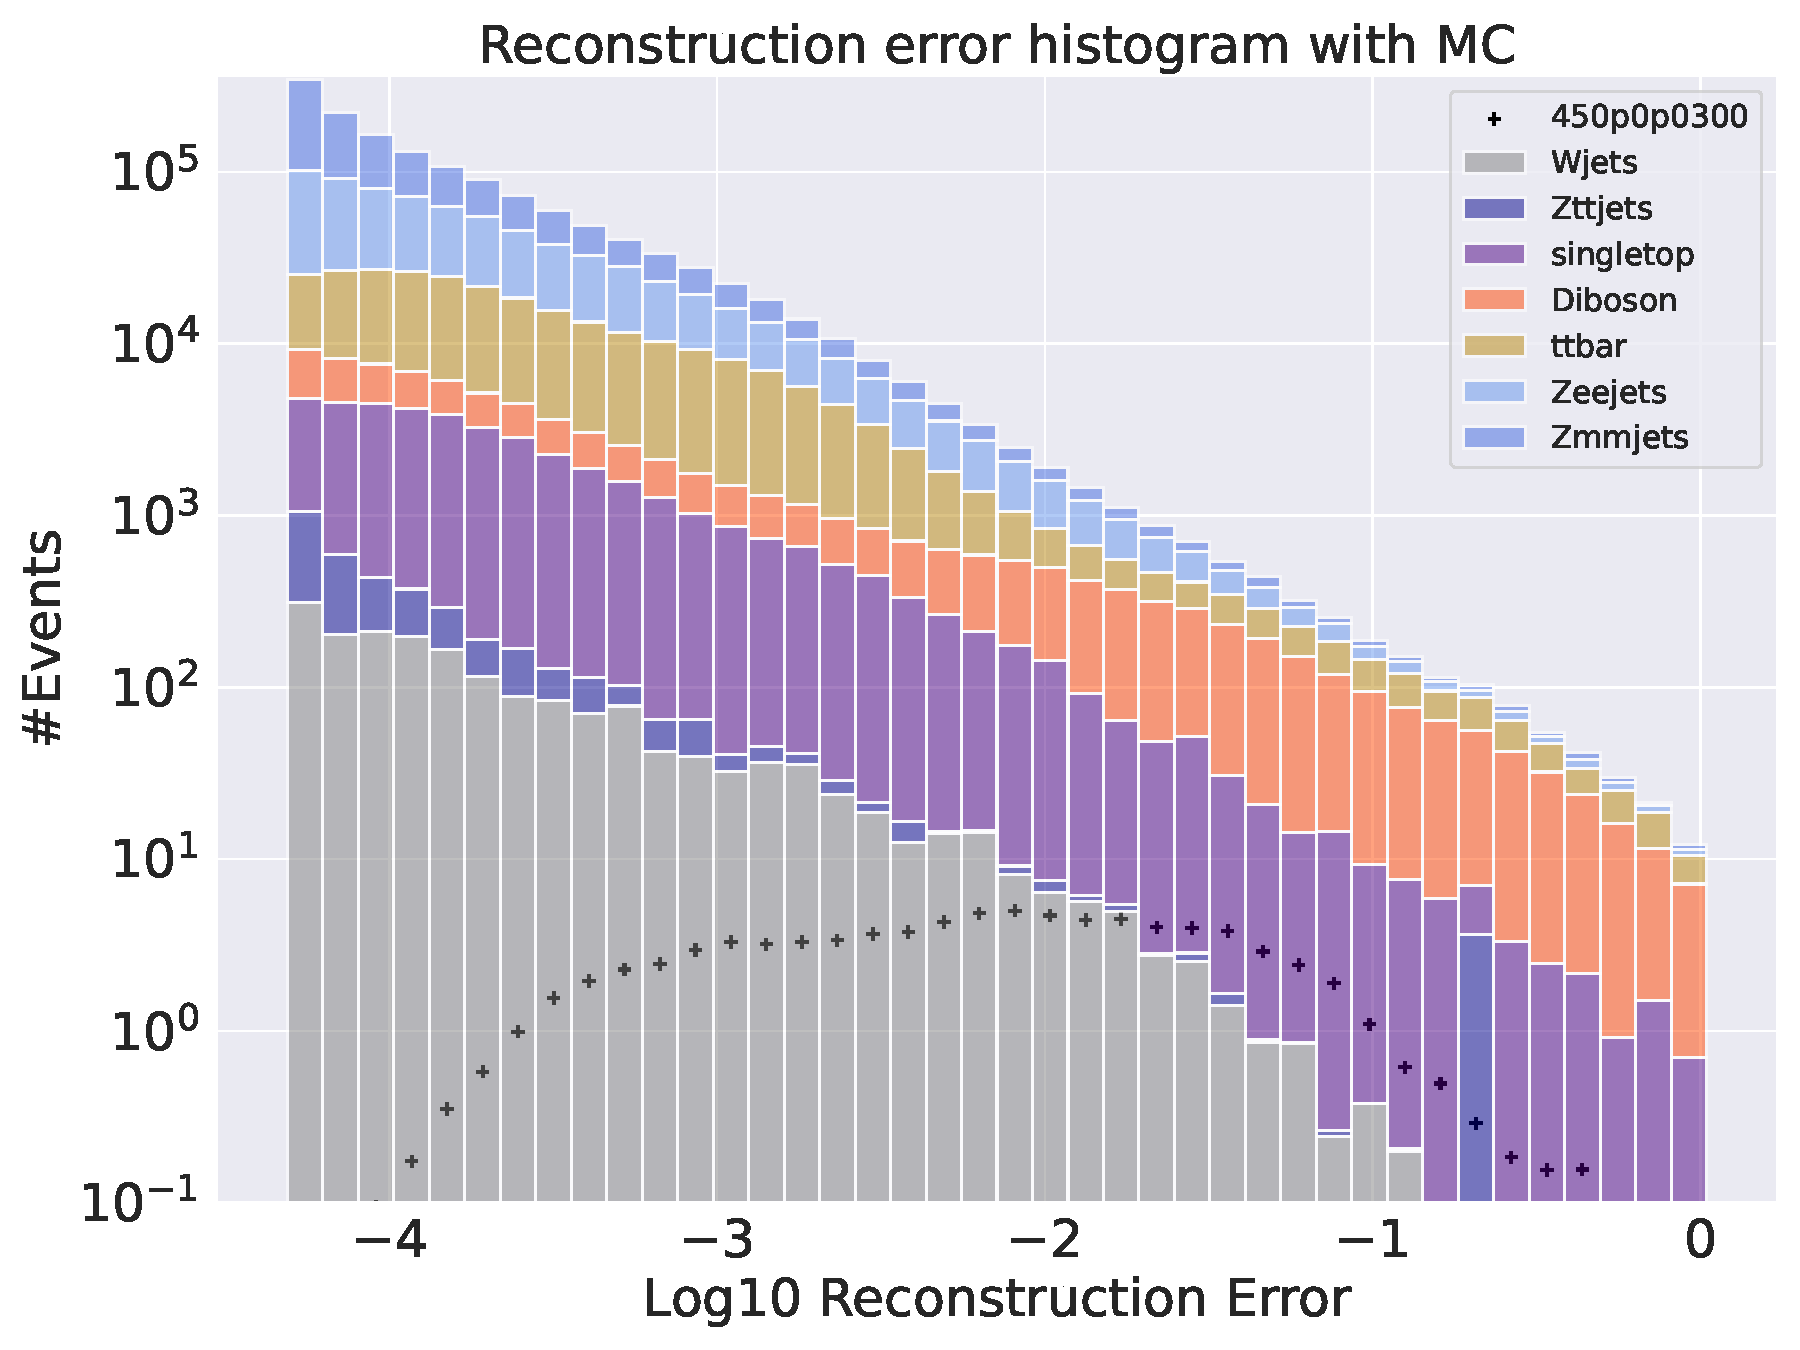
\includegraphics[width=\textwidth]{Figures/AE_testing/small/2lep/b_data_recon_big_rm3_feats_sig_450p0p0300_.pdf}
        \caption{ }
        \label{fig:AE_2lep_big_450}
    \end{subfigure}
    \hfill
    \begin{subfigure}{.60\textwidth}
        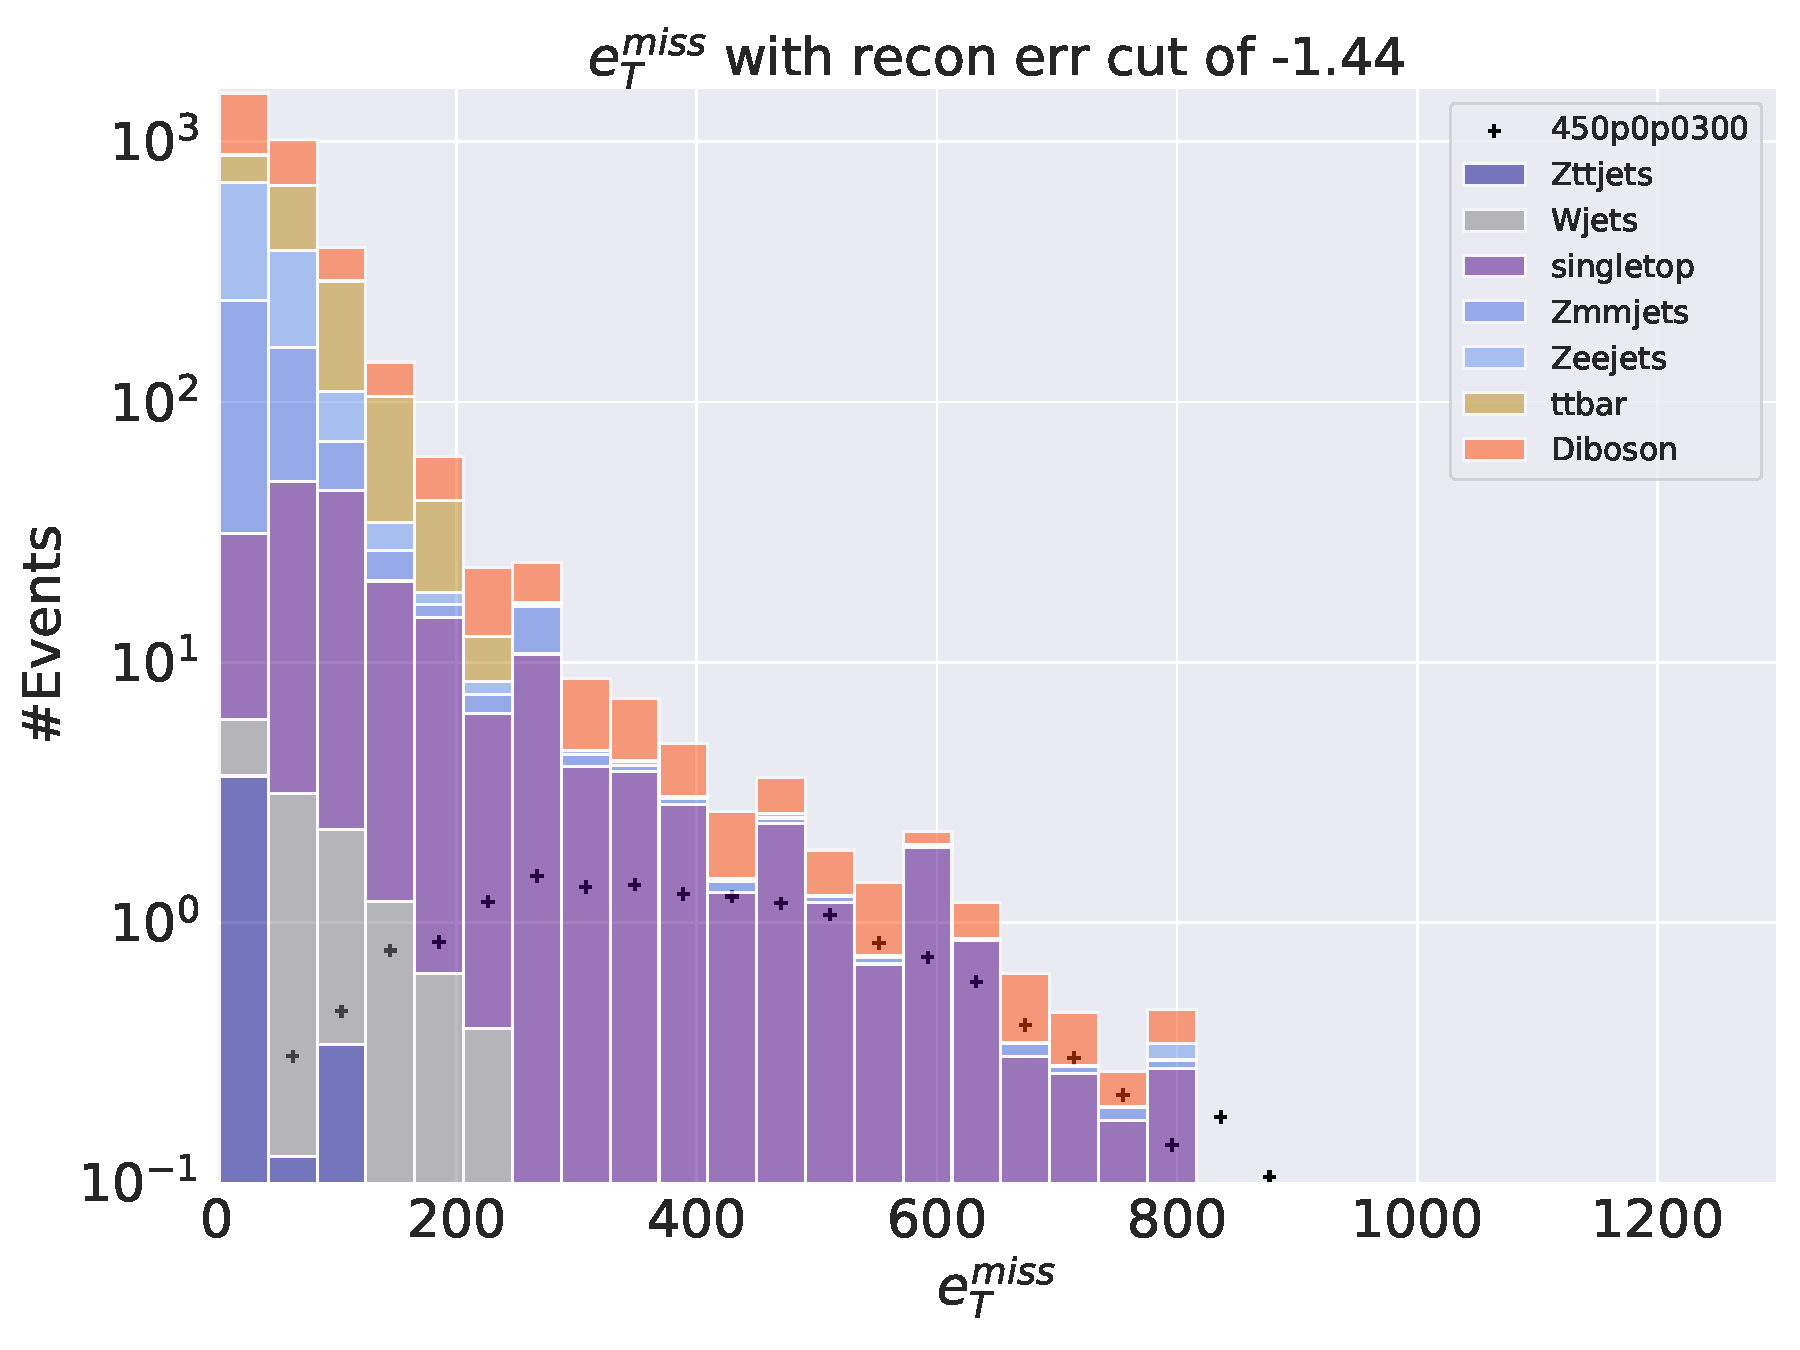
\includegraphics[width=\textwidth]{Figures/AE_testing/big/2lep/b_data_recon_big_rm3_feats_sig_450p0p0300_recon_errcut_-1.44.pdf}
        \caption{}
        \label{fig:AE_2lep_big_etmiss_450}
    \end{subfigure}
    \hfill 
    \begin{subfigure}{.60\textwidth}
        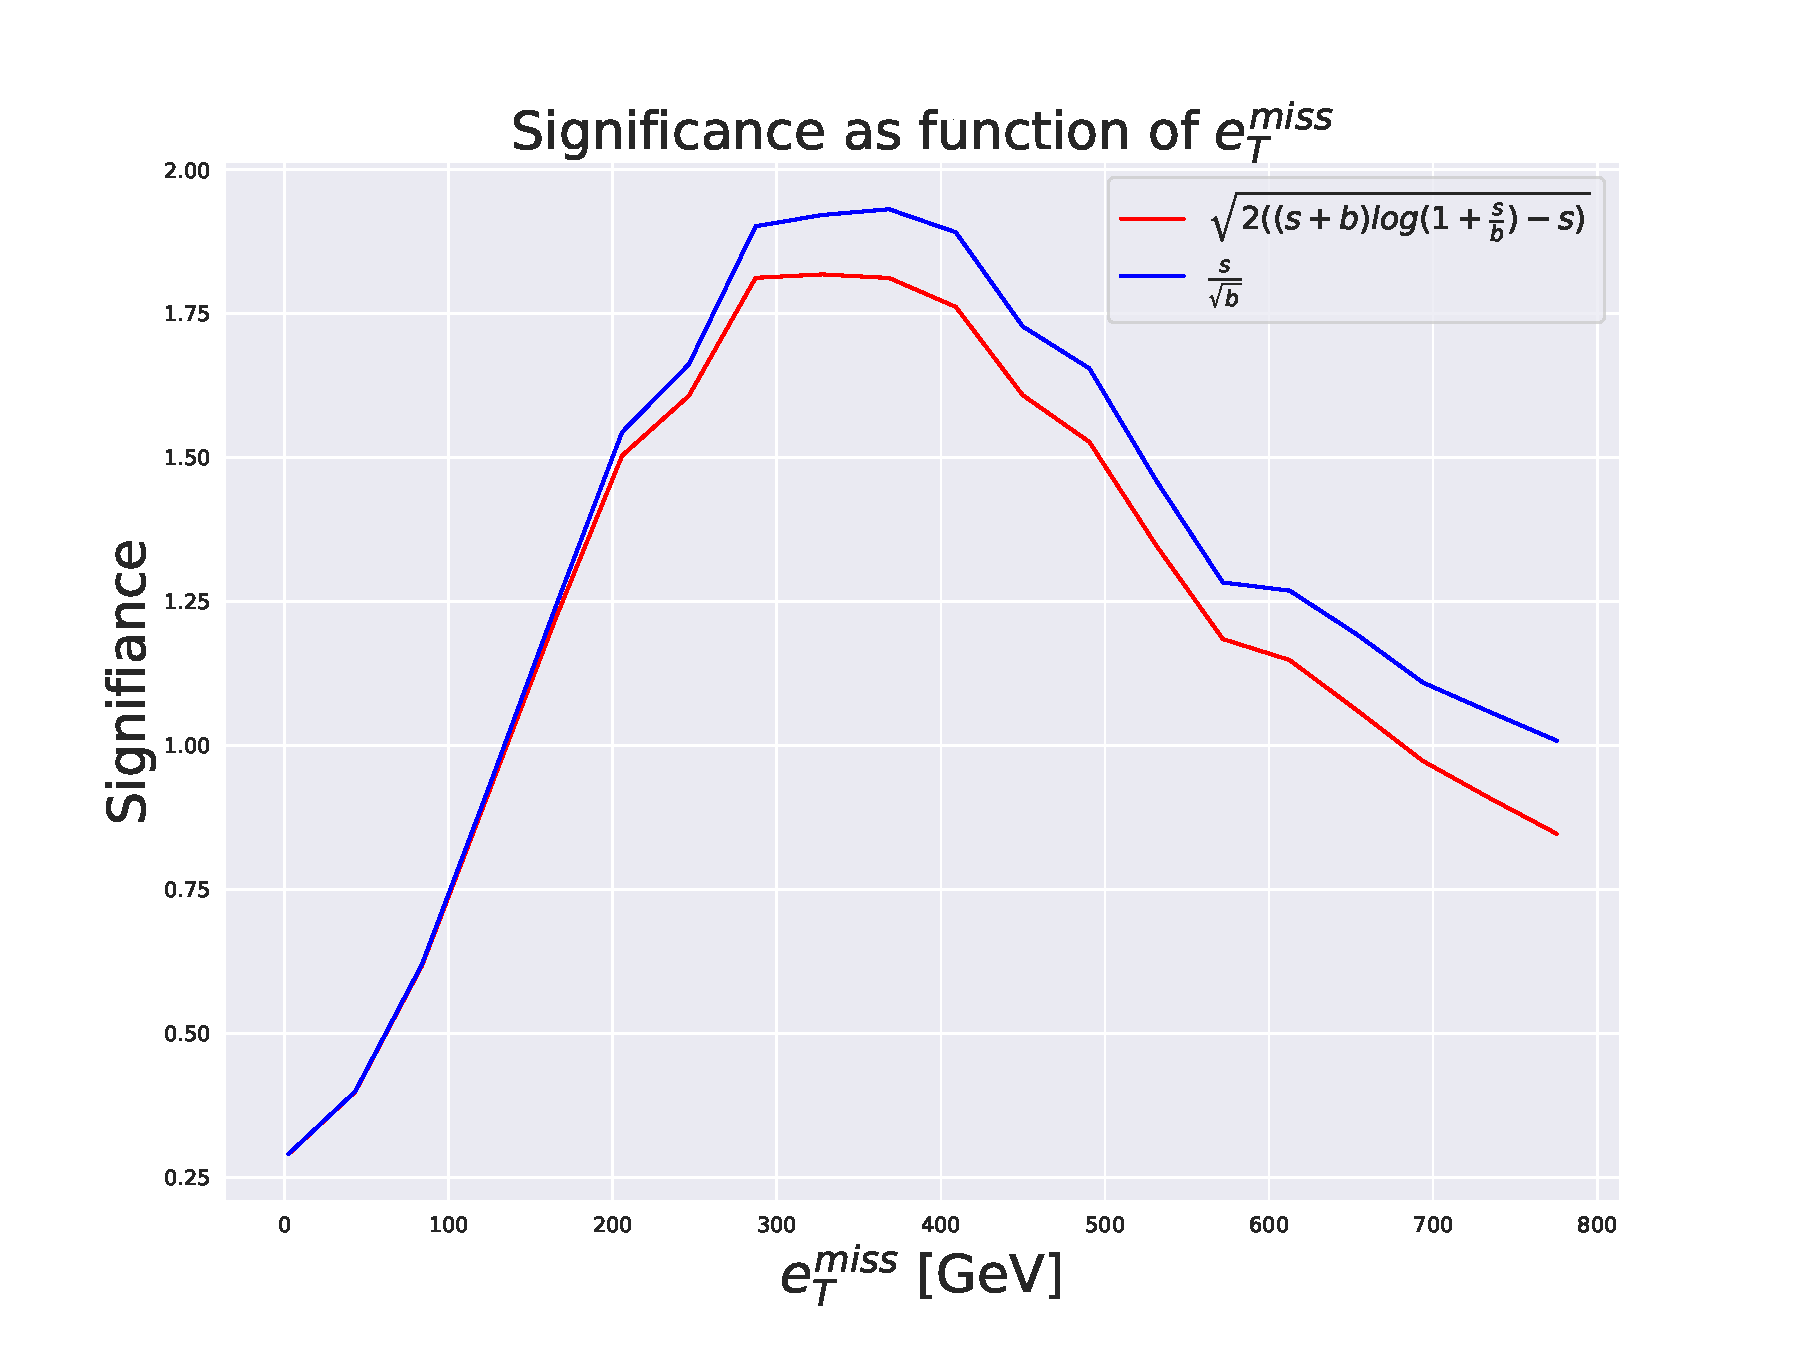
\includegraphics[width=\textwidth]{Figures/AE_testing/big/2lep/significance_etmiss_450p0p0300_-1.4360553938127363.pdf}
        \caption{}
        \label{fig:AE_2lep_big_signi_450}
    \end{subfigure}
    \hfill      
    \caption[2lep deep network | $450p300$ | AE]{Reconstruction error, $e_T^{miss}$ signal region, $m_{lll}$ signal region and significance as function of 
    $e_T^{miss}$ for the deep regular autoencoder using SUSY $450p300$.}
    \label{fig:AE_2lep_big_rec_sig_signi_450}
\end{figure}

\begin{figure}[H]
    \centering
    \begin{subfigure}{.60\textwidth}
        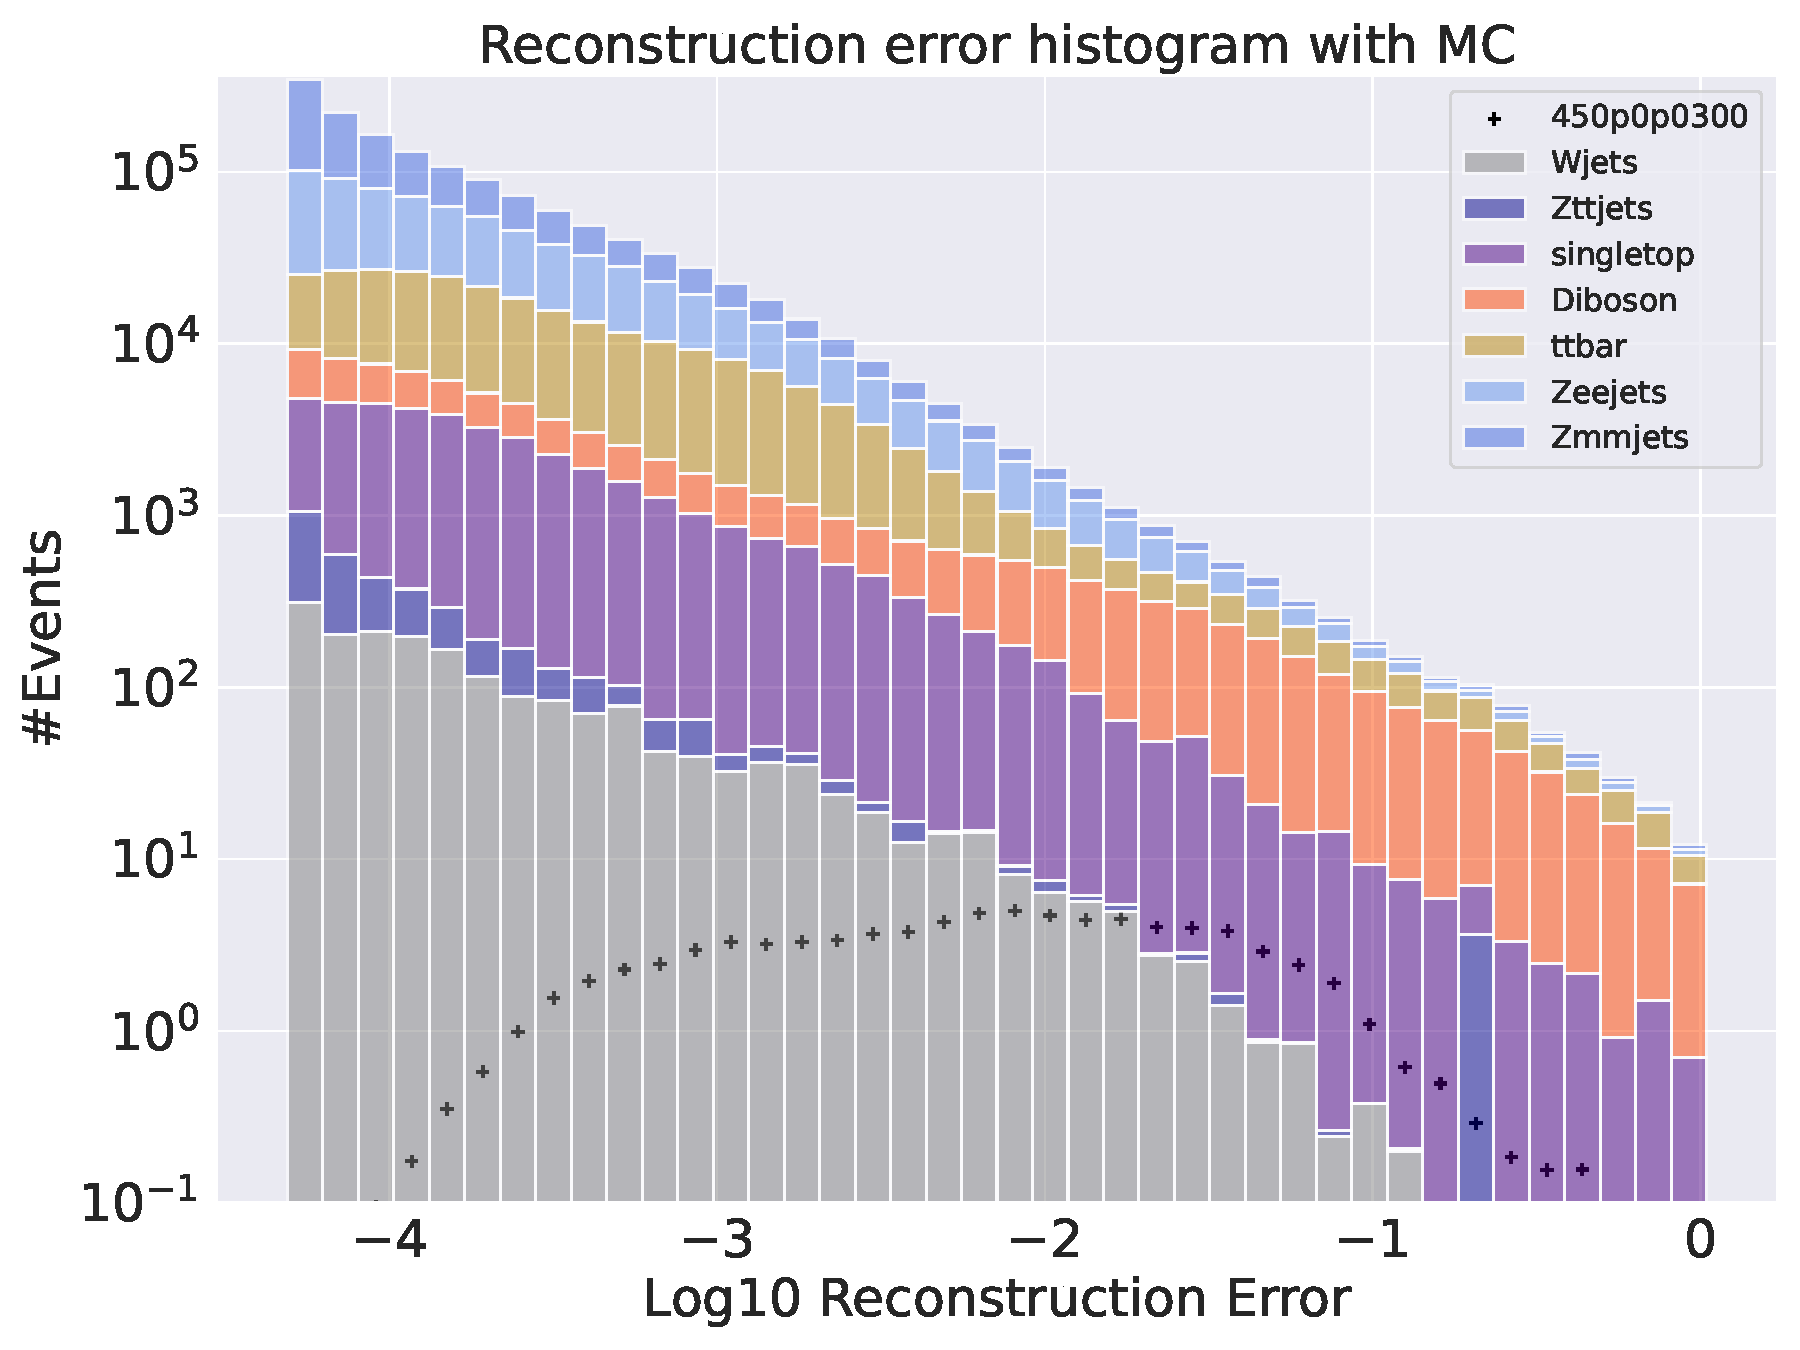
\includegraphics[width=\textwidth]{Figures/AE_testing/small/2lep/b_data_recon_big_rm3_feats_sig_450p0p0300_.pdf}
        \caption{ }
        \label{fig:AE_2lep_small_450}
    \end{subfigure}
    \hfill
    \begin{subfigure}{.60\textwidth}
        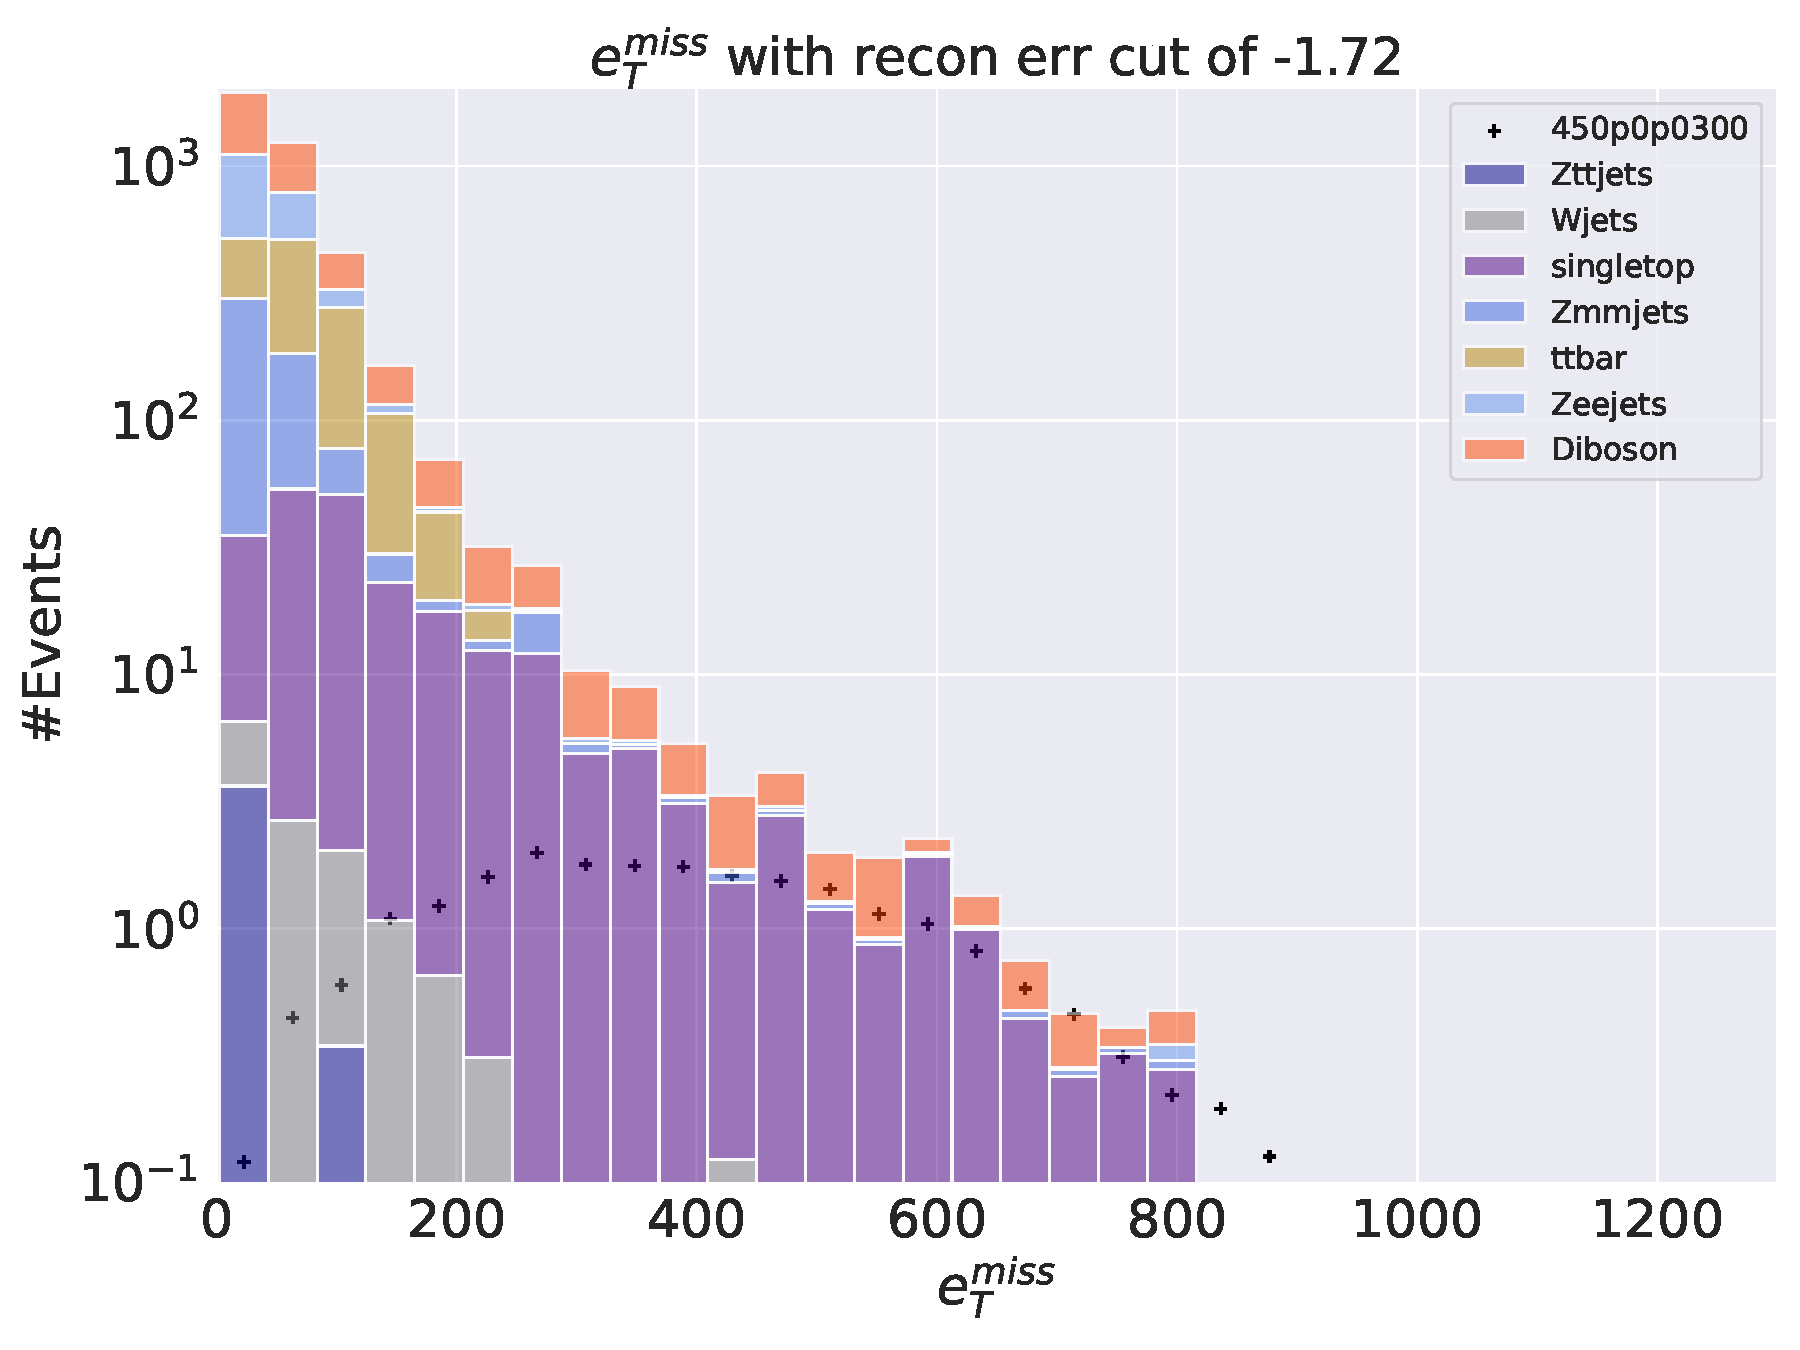
\includegraphics[width=\textwidth]{Figures/AE_testing/small/2lep/b_data_recon_big_rm3_feats_sig_450p0p0300_recon_errcut_-1.72.pdf}
        \caption{}
        \label{fig:AE_2lep_small_etmiss_450}
    \end{subfigure}
    \hfill  
    \begin{subfigure}{.60\textwidth}
        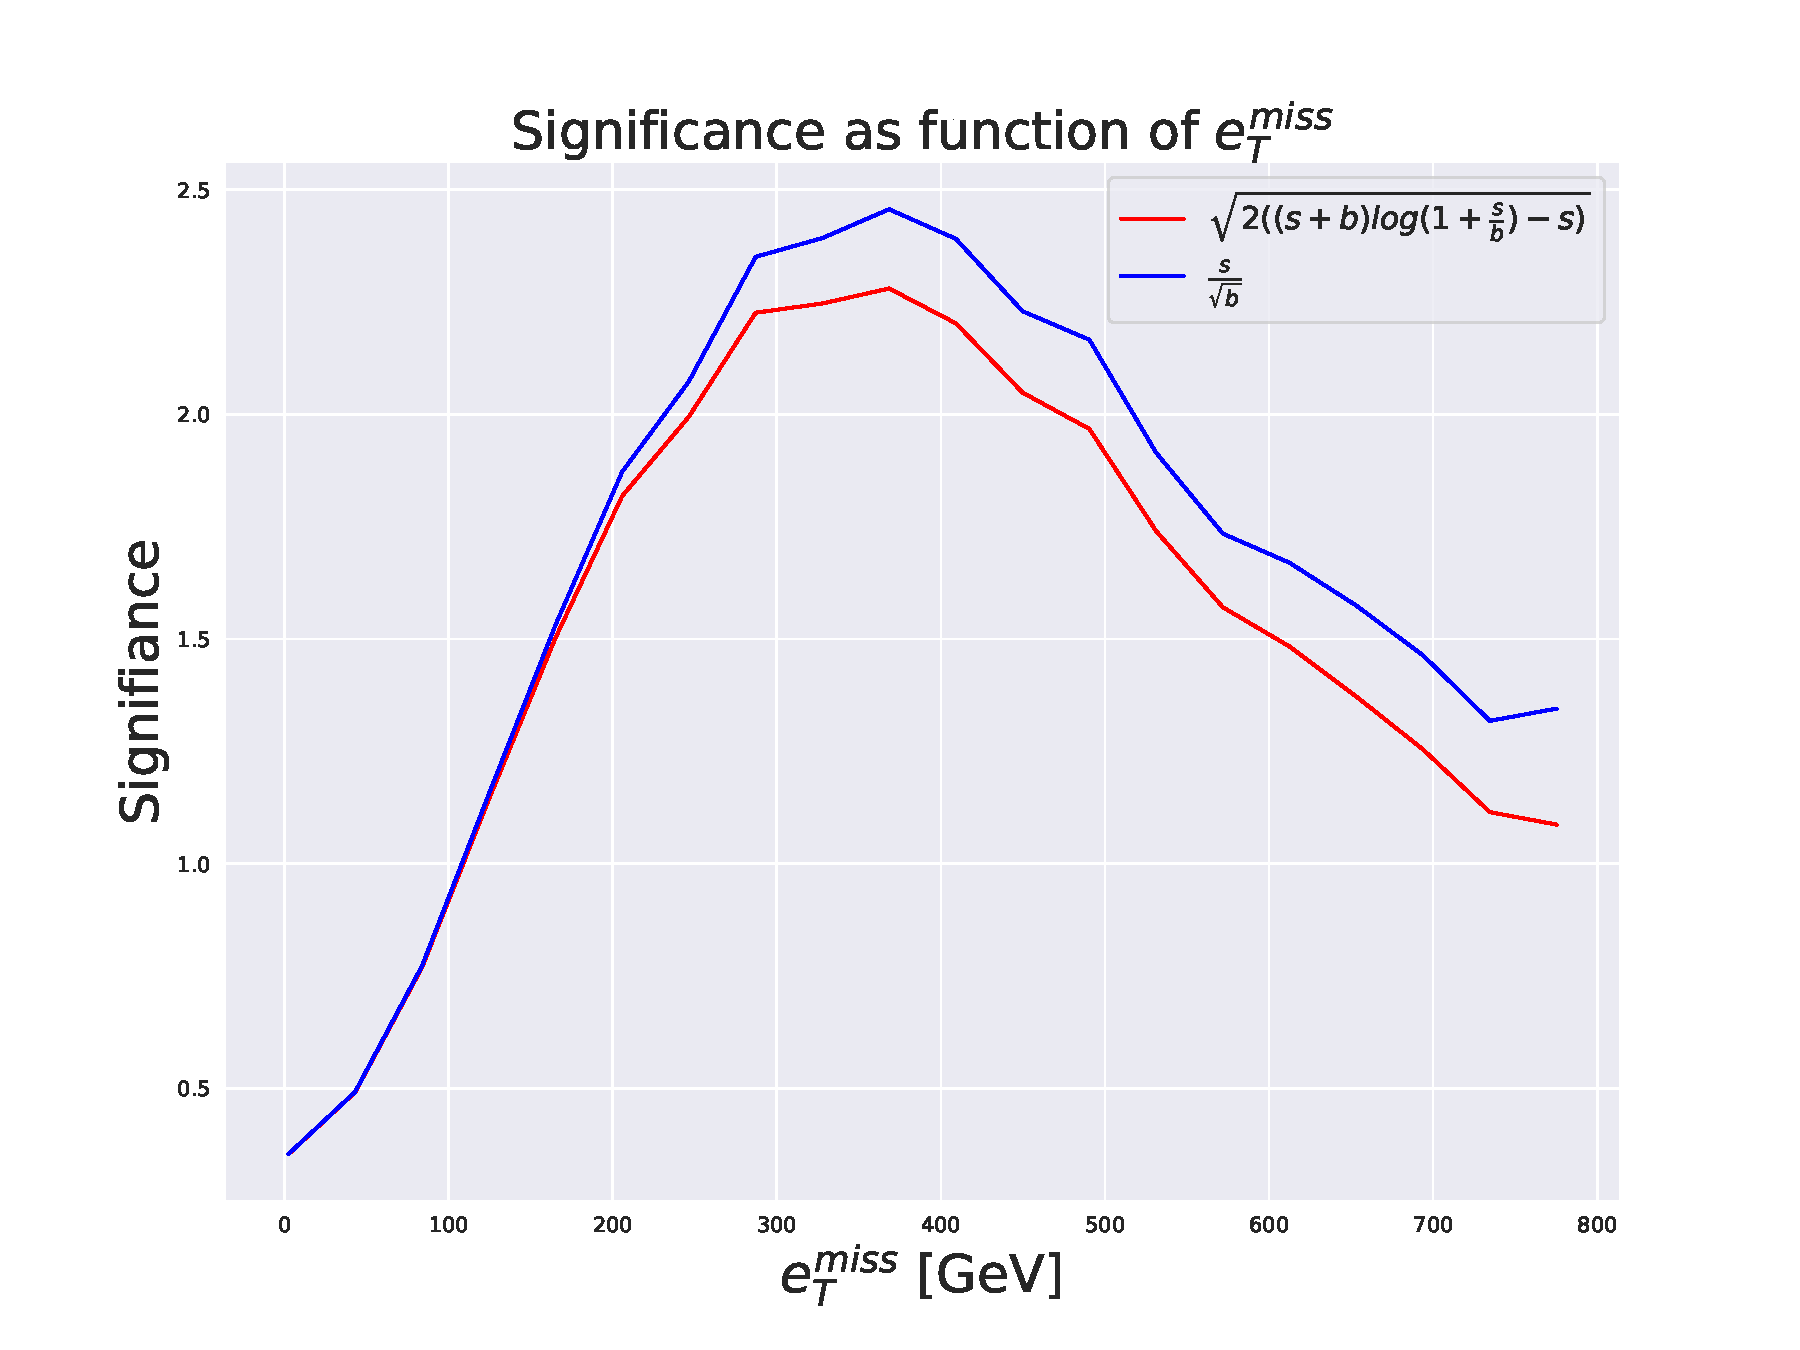
\includegraphics[width=\textwidth]{Figures/AE_testing/small/2lep/significance_etmiss_450p0p0300_-1.7167506533614734.pdf}
        \caption{}
        \label{fig:AE_2lep_small_signi_450}
    \end{subfigure}
    \hfill      
    \caption[2lep shallow network | $450p300$ | AE]{Reconstruction error, $e_T^{miss}$ signal region, $m_{lll}$ signal region and significance as function of 
    $e_T^{miss}$ for the deep regular autoencoder using SUSY $450p300$.}
    \label{fig:AE_2lep_small_rec_sig_signi_450}
\end{figure}


\begin{figure}[H]
    \centering
    \begin{subfigure}{.60\textwidth}
        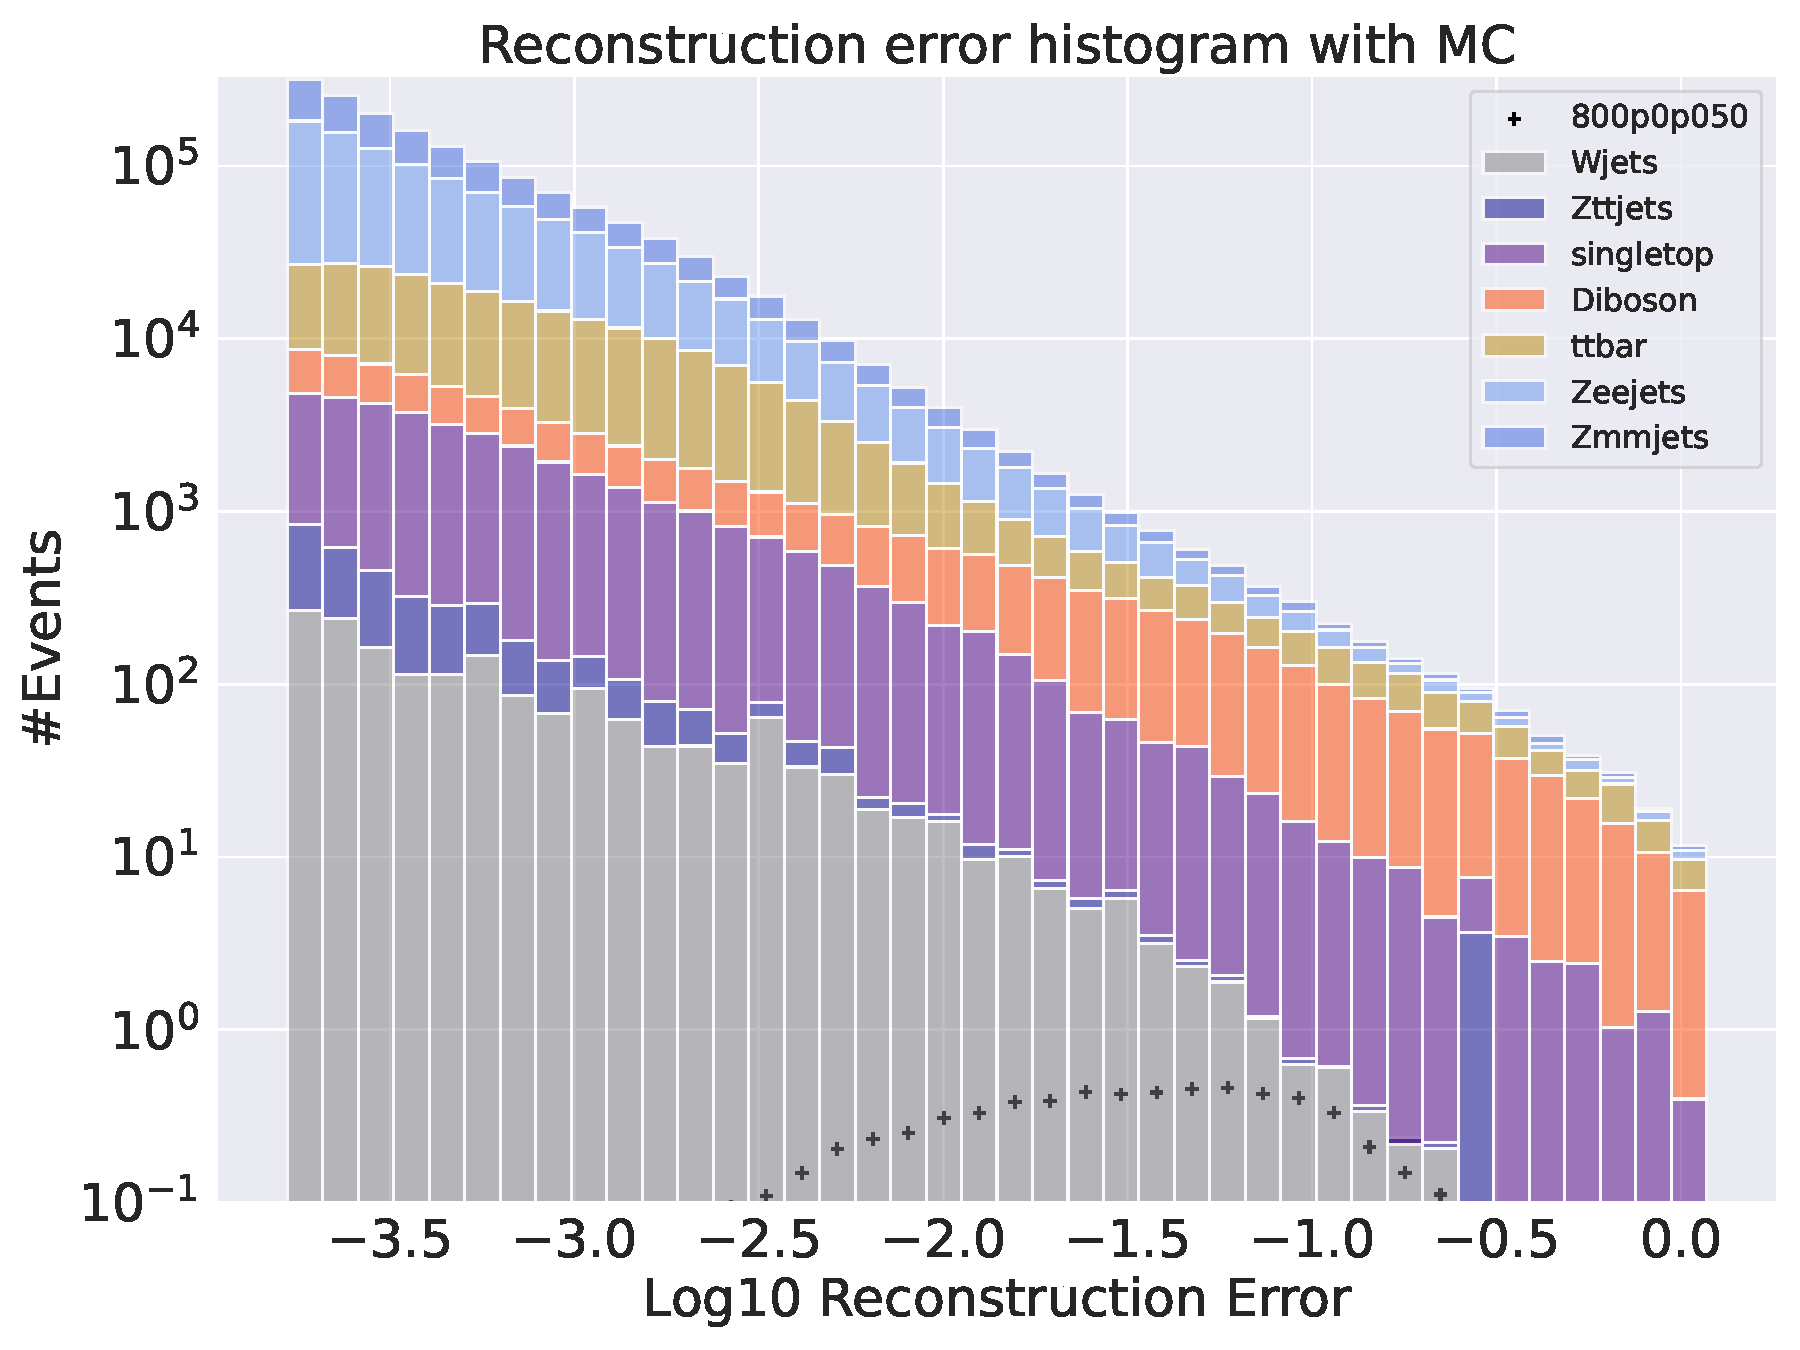
\includegraphics[width=\textwidth]{Figures/AE_testing/big/2lep/b_data_recon_big_rm3_feats_sig_800p0p050_.pdf}
        \caption{ }
        \label{fig:AE_2lep_big_800}
    \end{subfigure}
    \hfill
    \begin{subfigure}{.60\textwidth}
        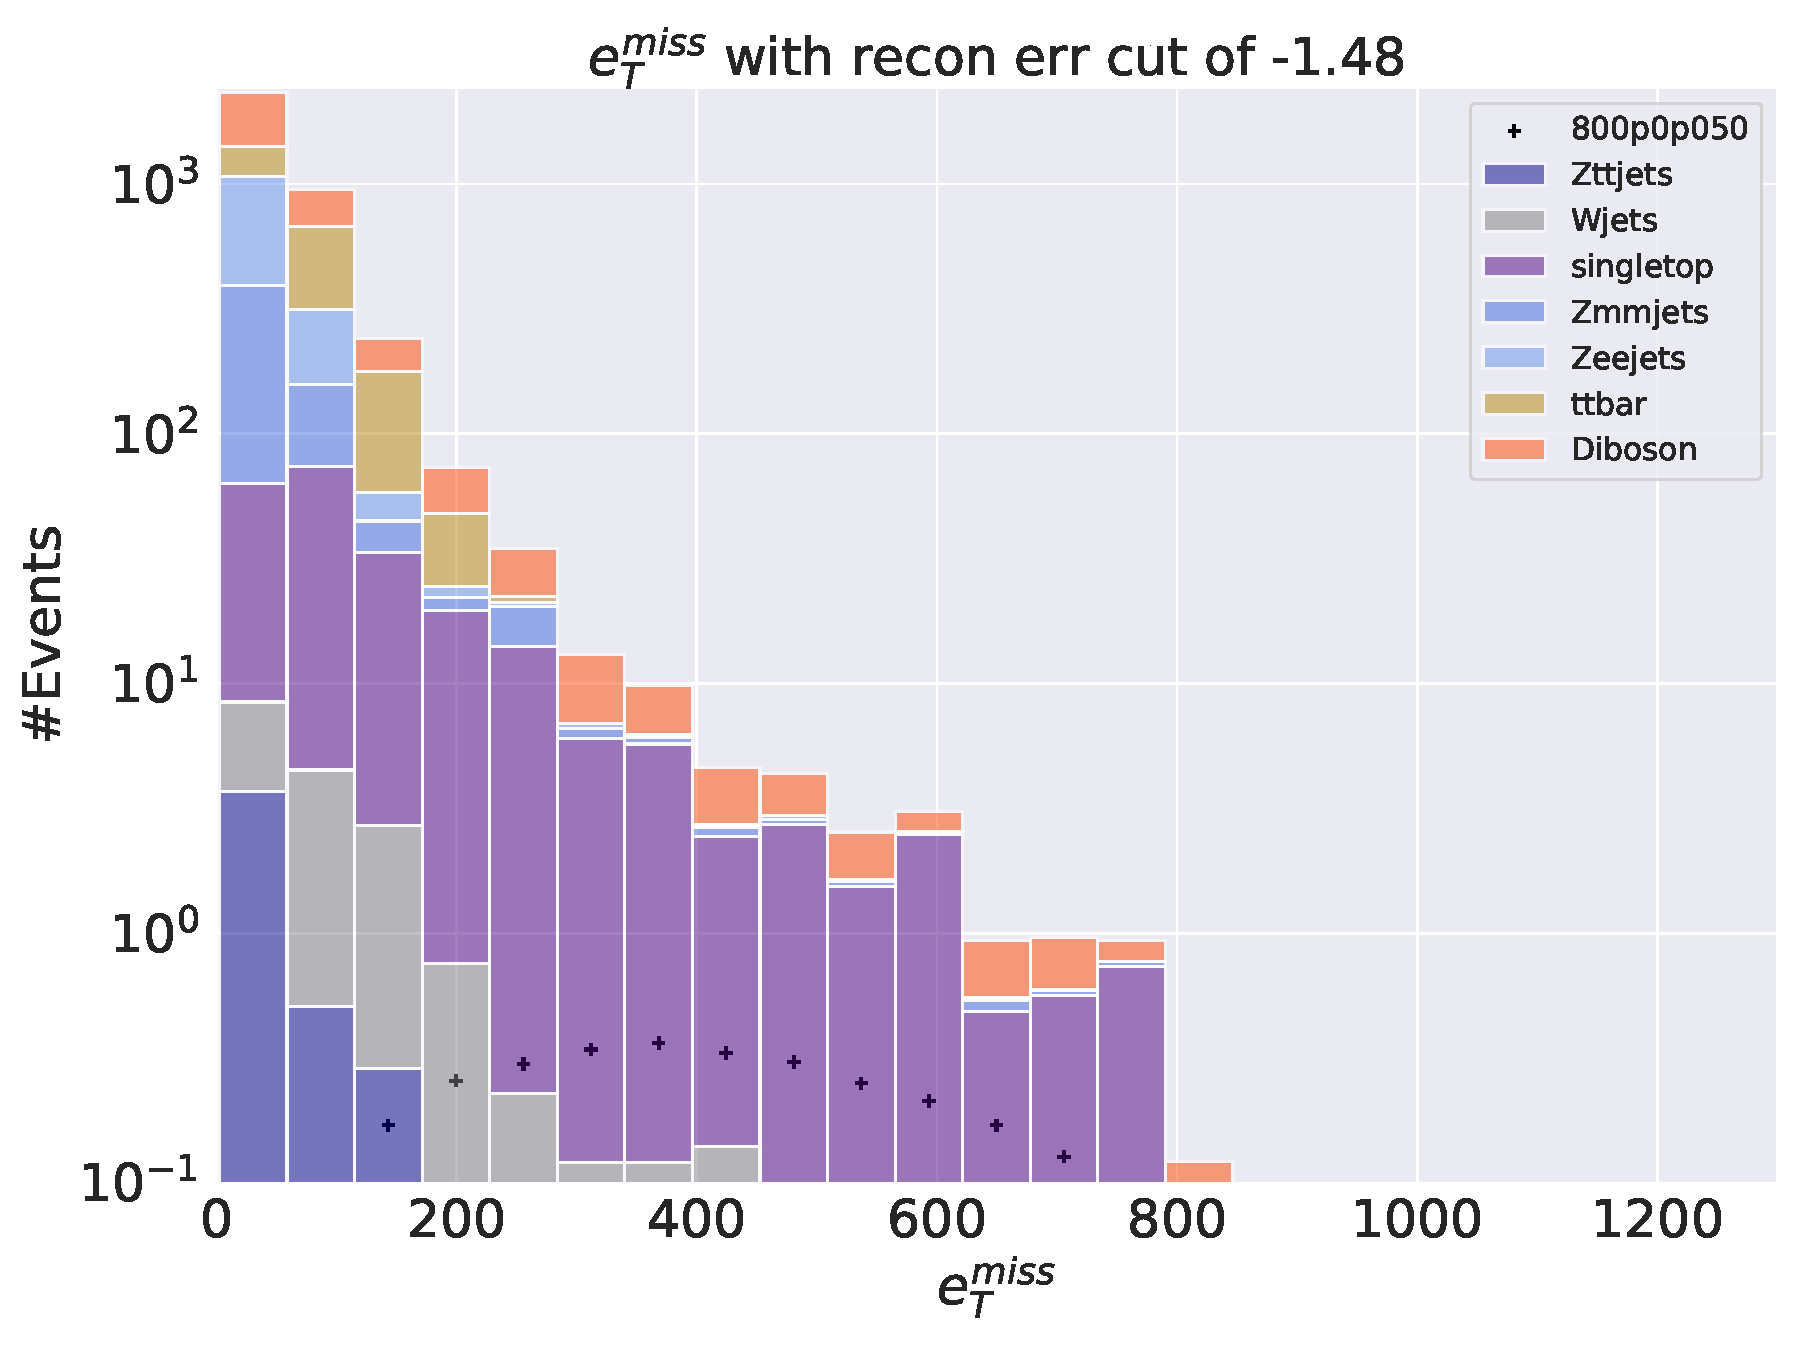
\includegraphics[width=\textwidth]{Figures/AE_testing/big/2lep/b_data_recon_big_rm3_feats_sig_800p0p050_recon_errcut_-1.48.pdf}
        \caption{}
        \label{fig:AE_2lep_big_etmiss_800}
    \end{subfigure}
    \hfill
      
    \begin{subfigure}{.60\textwidth}
        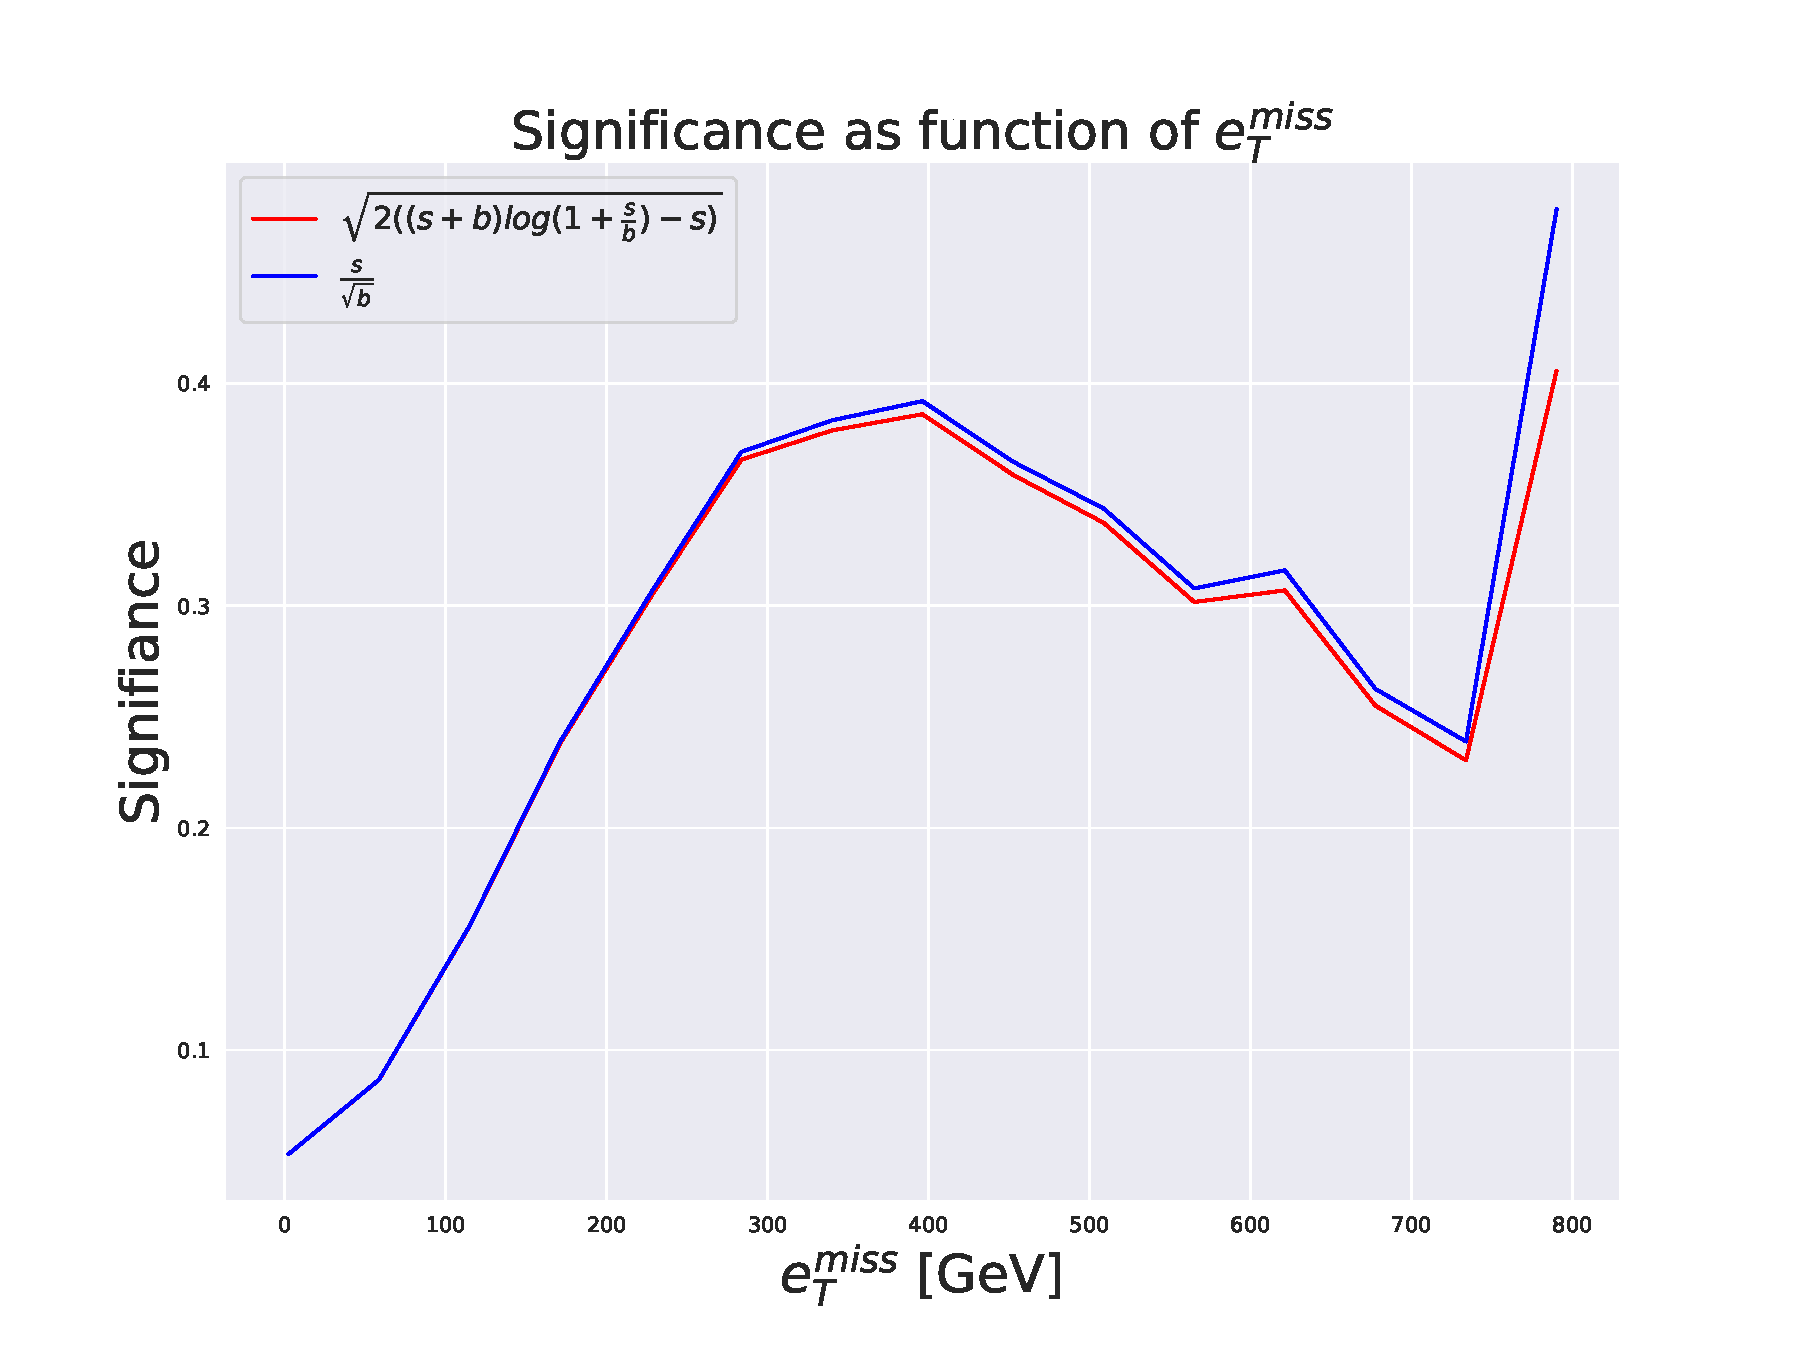
\includegraphics[width=\textwidth]{Figures/AE_testing/big/2lep/significance_etmiss_800p0p050_-1.4833711230716062.pdf}
        \caption{}
        \label{fig:AE_2lep_big_signi_800}
    \end{subfigure}
    \hfill      
    \caption[2lep deep network | $800p50$ | AE]{Reconstruction error, $e_T^{miss}$ signal region, $m_{lll}$ signal region and significance as function of 
    $e_T^{miss}$ for the deep regular autoencoder using SUSY $800p50$.}
    \label{fig:AE_2lep_big_rec_sig_signi_800}
\end{figure}

\begin{figure}[H]
    \centering
    \begin{subfigure}{.60\textwidth}
        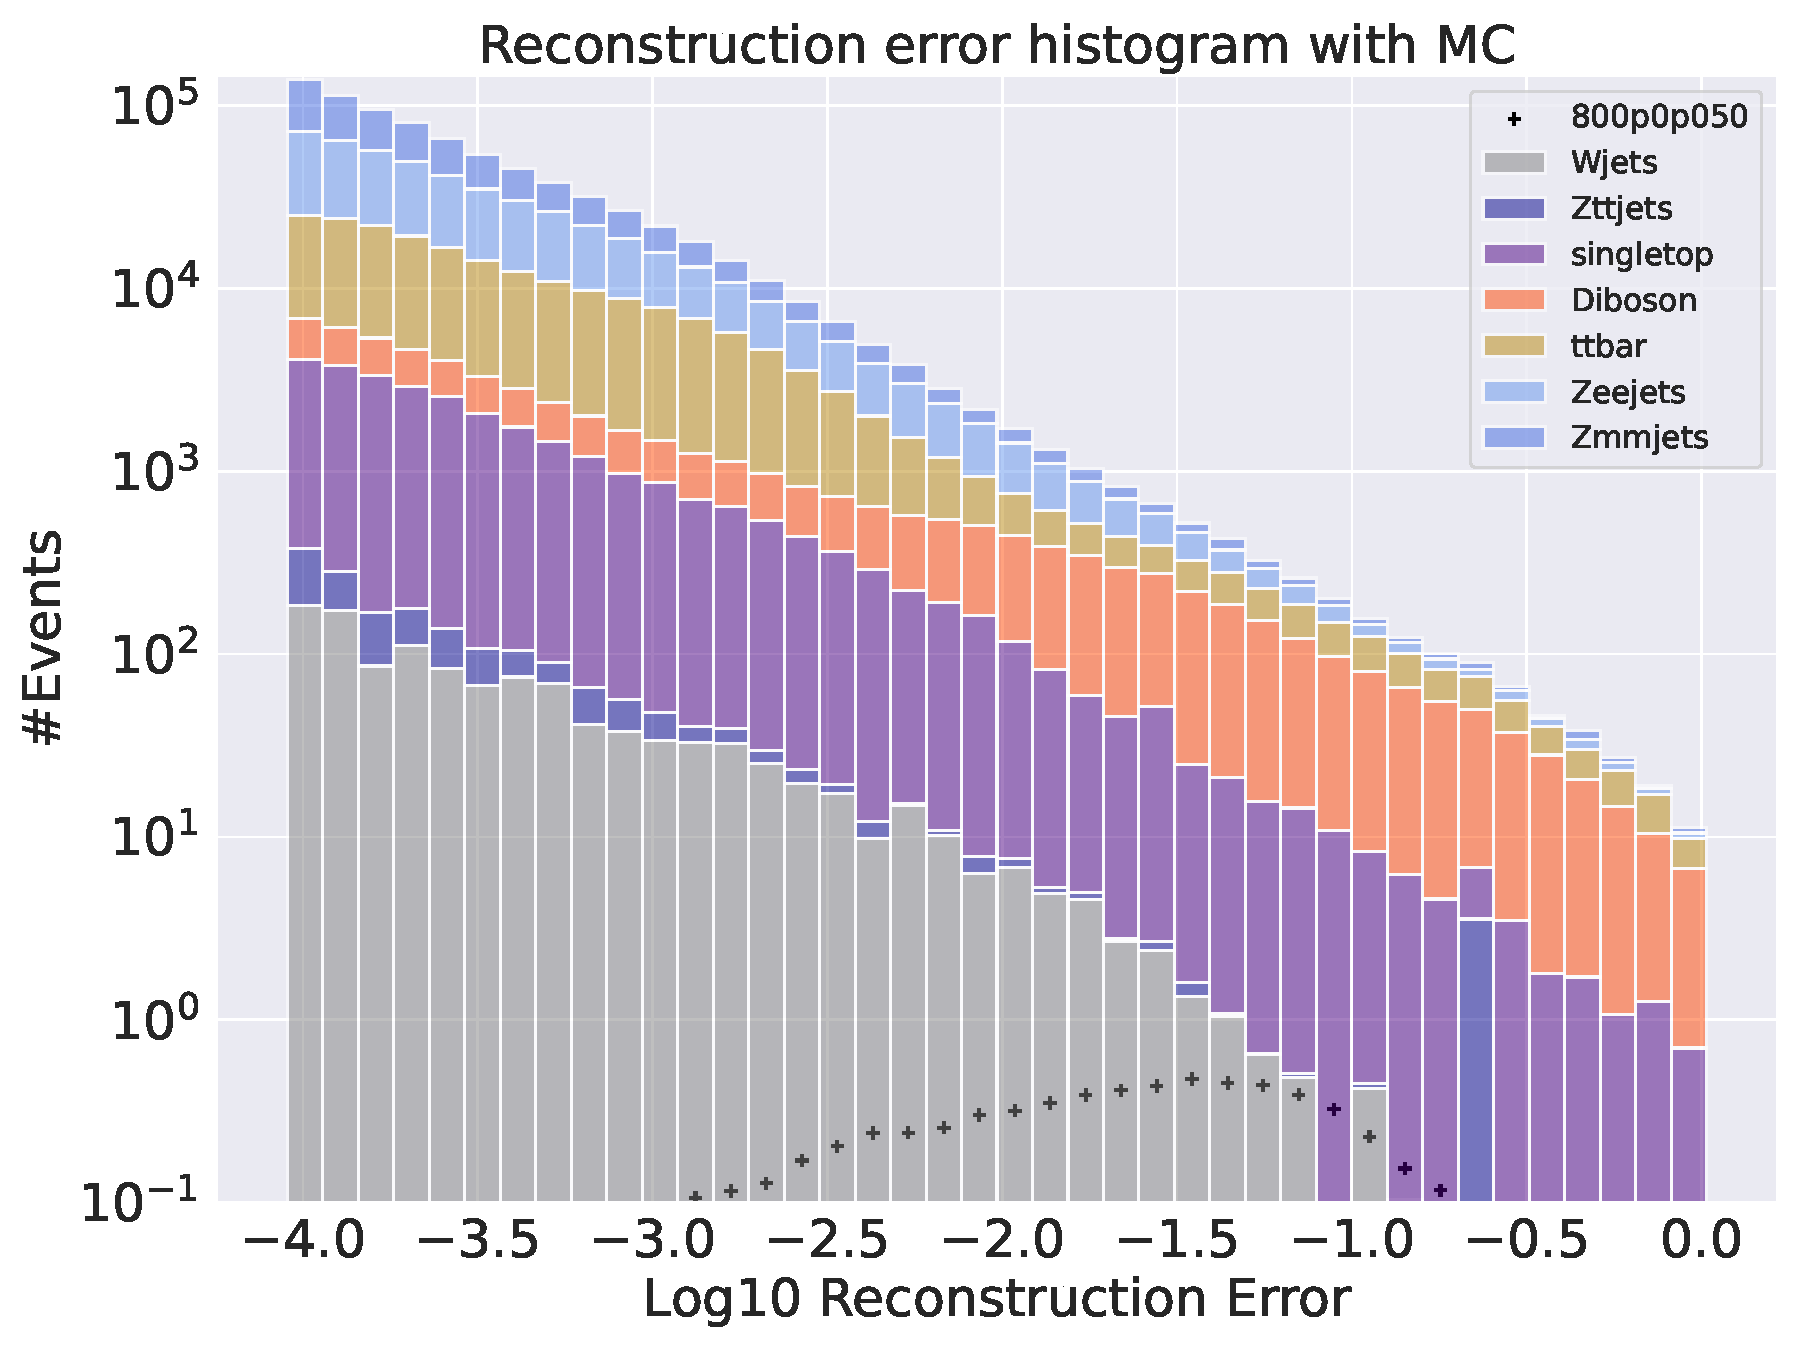
\includegraphics[width=\textwidth]{Figures/AE_testing/small/2lep/b_data_recon_big_rm3_feats_sig_800p0p050_.pdf}
        \caption{ }
        \label{fig:AE_2lep_small_800}
    \end{subfigure}
    \hfill
    \begin{subfigure}{.60\textwidth}
        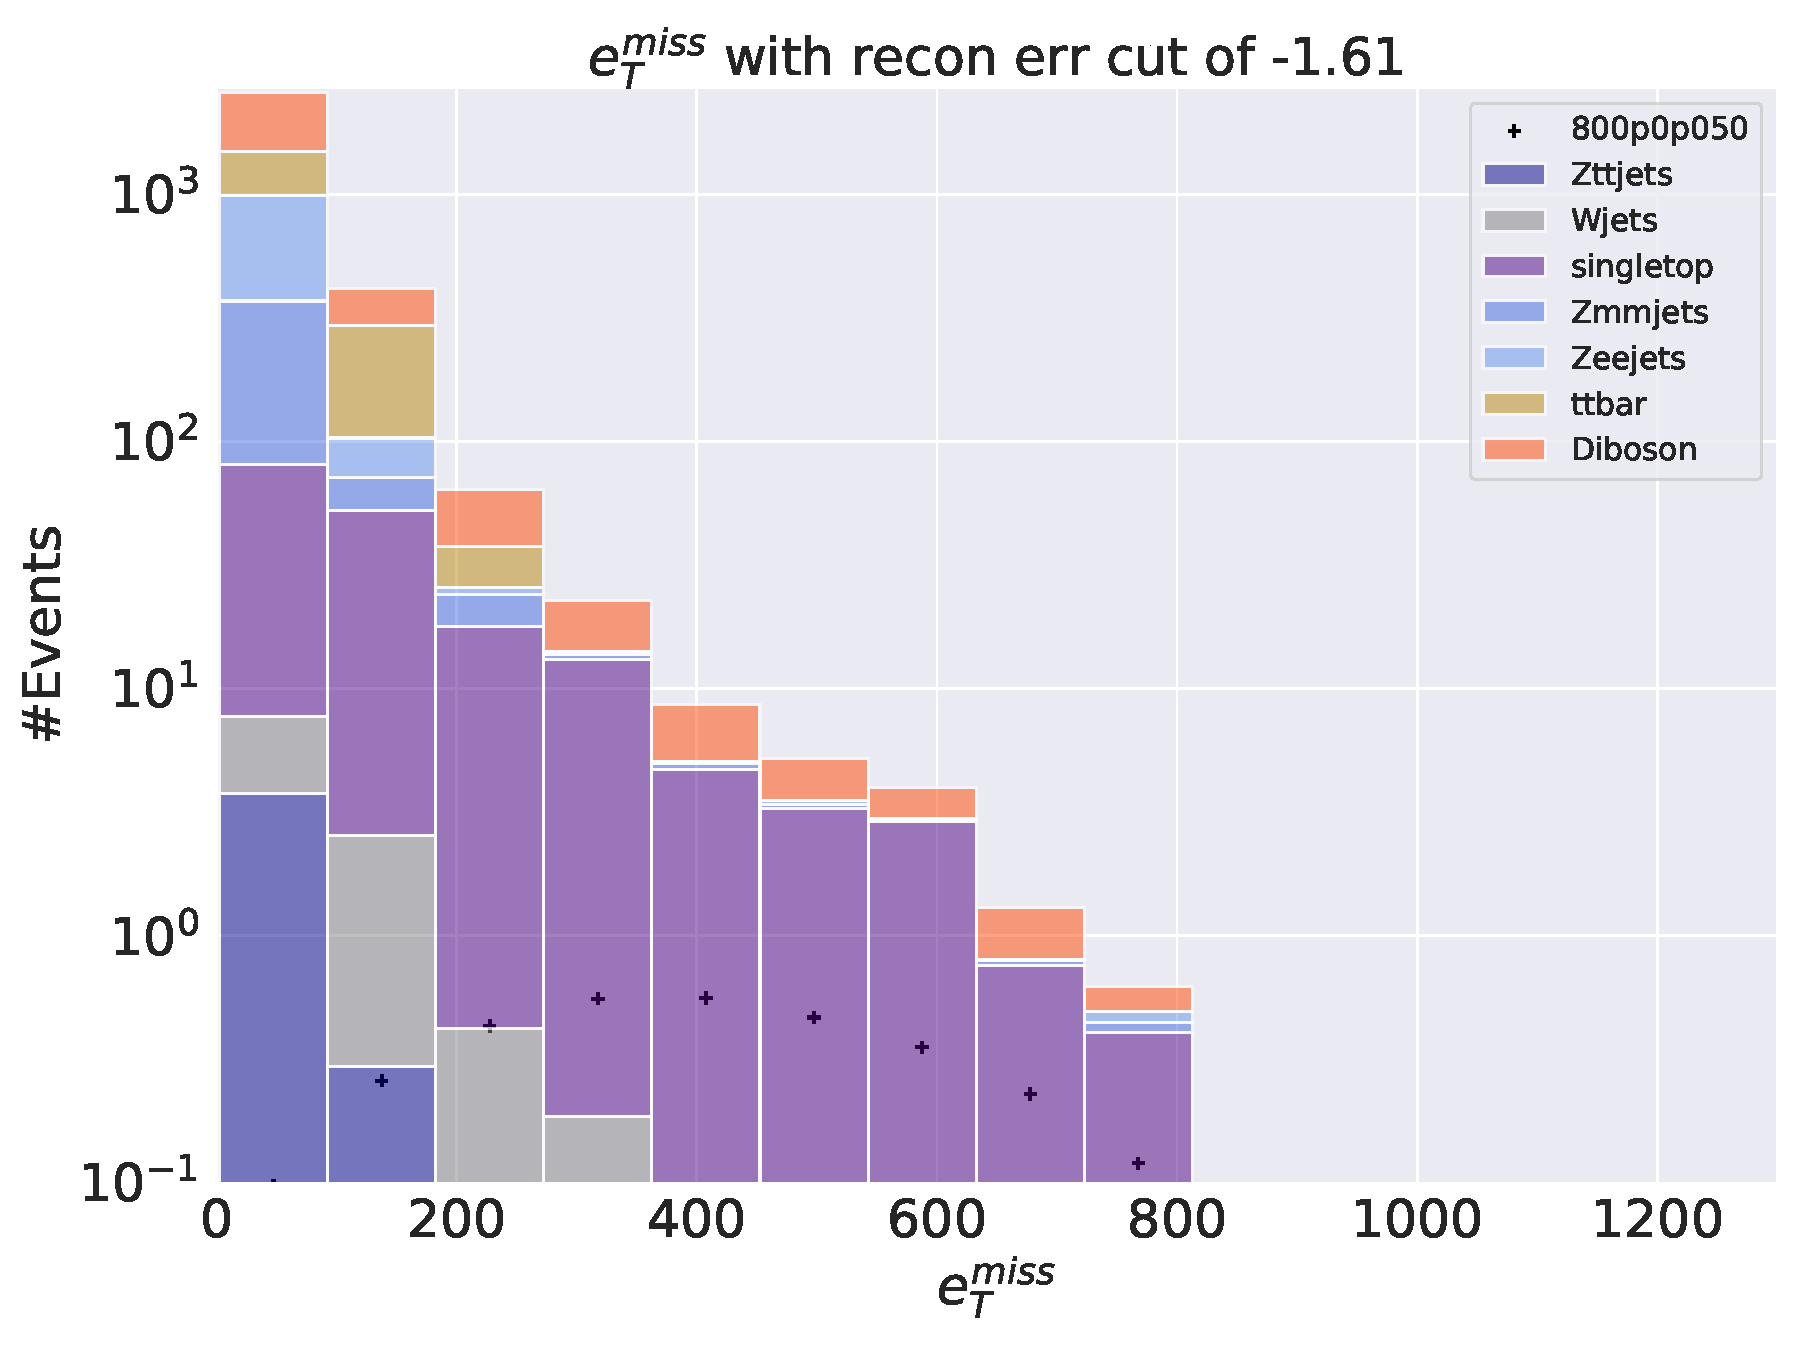
\includegraphics[width=\textwidth]{Figures/AE_testing/small/2lep/b_data_recon_big_rm3_feats_sig_800p0p050_recon_errcut_-1.61.pdf}
        \caption{}
        \label{fig:AE_2lep_small_etmiss_800}
    \end{subfigure}
    \hfill  
    \begin{subfigure}{.60\textwidth}
        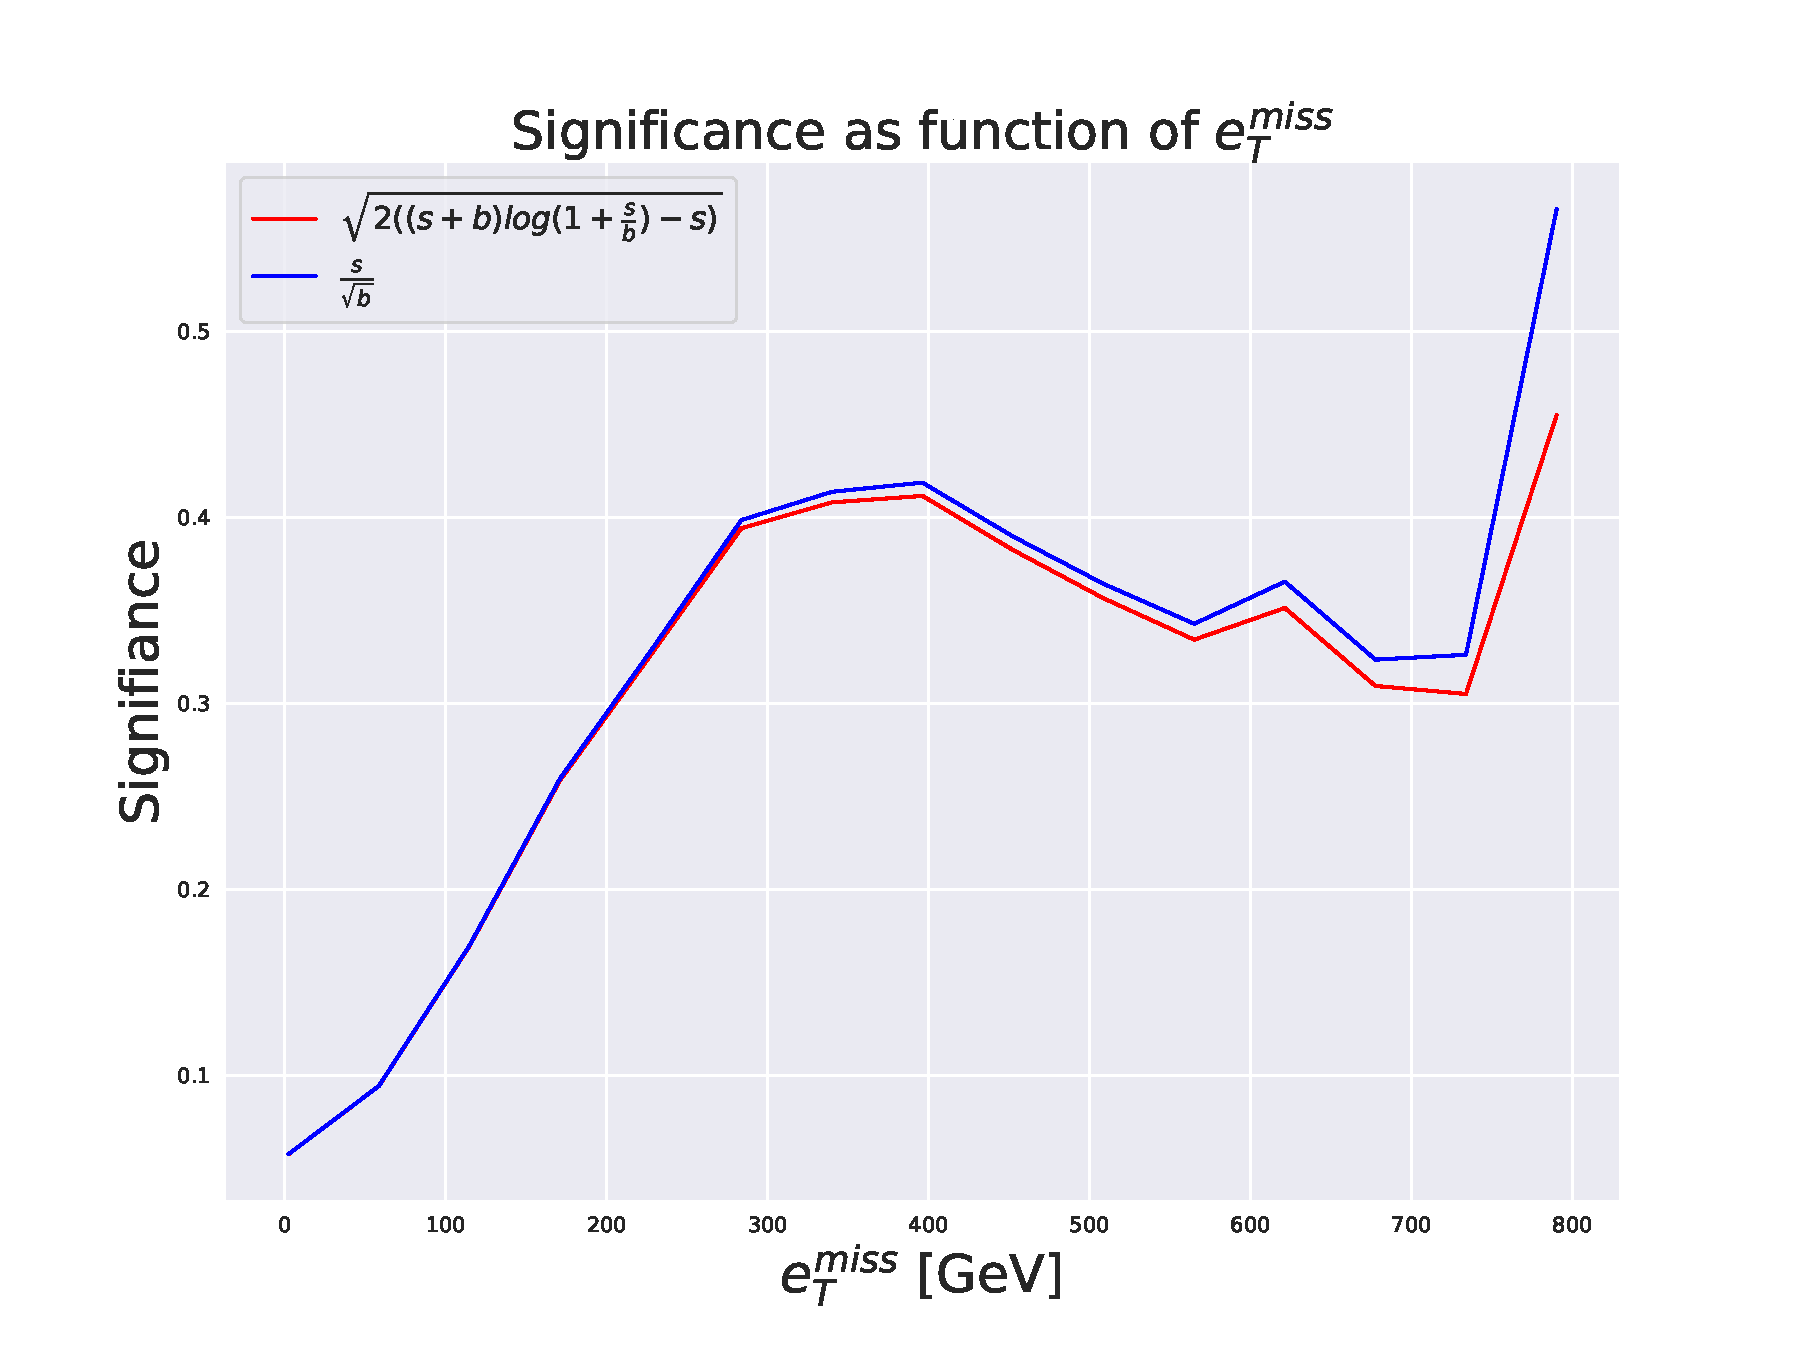
\includegraphics[width=\textwidth]{Figures/AE_testing/small/2lep/significance_etmiss_800p0p050_-1.6117055611472277.pdf}
        \caption{}
        \label{fig:AE_2lep_small_signi_800}
    \end{subfigure}
    \hfill      
    \caption[2lep shallow network | $800p50$ | AE]{Reconstruction error, $e_T^{miss}$ signal region, $m_{lll}$ signal region and significance as function of 
    $e_T^{miss}$ for the shallow regular autoencoder using SUSY $800p50$.}
    \label{fig:AE_2lep_small_rec_sig_signi_800}
\end{figure}


In figures \ref{fig:AE_2lep_big_rec_sig_signi_450}, \ref{fig:AE_2lep_small_rec_sig_signi_450}, 
\ref{fig:AE_2lep_big_rec_sig_signi_800} and \ref{fig:AE_2lep_small_rec_sig_signi_800} we have three 
subplots containing the total reconstruction error distributions, the $e_T^{miss}$ signal region, 
and the significance as function of $e_T^{miss}$ curve respectively. They were created using 
the shallow and deep regular autoencoder with the 2 lepton + $e_T^{miss}$ dataset.
In figures \ref{fig:AE_2lep_big_450}, \ref{fig:AE_2lep_small_450}, \ref{fig:AE_2lep_big_800}, 
\ref{fig:AE_2lep_small_800} we observe that there is a general trend here for both the small 
and large regular autoencoder where the background distributions are highly shifted to the 
lower end of the reconstruction error range. This is a continuing trend following the 3 
lepton + $e_T^{miss}$ case shown in figures \ref{fig:AE_3lep_big_450}, \ref{fig:AE_3lep_small_450},
\ref{fig:AE_3lep_big_800}, \ref{fig:AE_3lep_small_800}. 
This indicates that as we increase the statistics, in other words the amount of background events 
used for training, the ability of the autoencoder to learn the internal structure increases. 
\hl{It is also interesting to observe here that as the reconstruction error increases, the amount 
of each sample in a given bin changes alot.} As expected, Zmmjets and Zeejets along with ttbar 
are the channels with the highest statistics in the 2 lepton + $e_T^{miss}$ dataset, thus it 
should be easier to learn to better reconstruct those events. However, note the amount of 
diboson in the higher end of the reconstruction error histograms, as well as in the $e_T^{miss}$ 
post reconstruction error cut distributions. One explanation for this could be the sample 
discrepency explained in section \ref{sec:mcdatacomp}. It would appear that too much of the 
diboson samples is cut, leading to not enough samples for it to appropriately learn the RMM 
structure for that channel, leading to the high reconstruction error values for some of 
those events. Note also here that the reconstruction threshold where this effect is getting 
more noticable around $10^{-2}$ and higer, where the events are on the order of a 1000 or 
less per bin. \hl{Thus, it is not alot of events, but still enough to note}. \par Using the signal 
region definition \hl{from above} we set cuts on the reconstruction error and then calculate the 
significance of the signal. \par
In figures \ref{fig:AE_2lep_big_etmiss_450}, \ref{fig:AE_2lep_small_etmiss_450}, \ref{fig:AE_2lep_big_etmiss_800} and  
\ref{fig:AE_2lep_small_etmiss_800} we have the $e_T^{miss}$ distributions for 
the least strict cuts for the regular autoencoder models. Now, one indication that the search strategy 
used in this thesis could work is if the models can improve the significance from just looking at 
the $e_T^{miss}$ distributions of the background and the signal in mind. Thus, we want to compare the pre 
reconstruction error significance with the signal region based on the autoencoder output. The significance 
in the pre reconstruction error case were for the SUSY $450p300$ signal 0.017 using both the small and large 
statistics formula, and 0.0014 for the SUSY $800p50$ signal. Note here that for $e_T^{miss}$, no physics 
informed cuts have been used, but there are certain cuts that can increase the significance, so the significance
in should be considered to possibly be somewhat higher. \par
From figures \ref{fig:AE_2lep_big_signi_450}, 
\ref{fig:AE_2lep_small_signi_450}, \ref{fig:AE_2lep_big_signi_800} and  \ref{fig:AE_2lep_small_signi_800} 
we have the significance as a function of $e_T^{miss}$ for both signals using the shallow and deep autoencoder. 
This graph shows how implementing another cut in the signal region, namely where in the $e_T^{miss}$ distribution 
to select event, allows for higher significance. We see here that the shallow autoencoder gets a significance of 
almost 2.5 in the SUSY $450p300$ case, being the highest score, and beating the pre reconstruction error significance 
by alot. Another interesting point to note here is the tail ends, especially for the SUSY $800p50$ signal. 
This model has some events of very high $e_T^{miss}$, and in the tail end, there might be very few or none 
background events. It should be noted that the significance for the $800p50$ signal model is a lot smaller than 
for the $450p300$ signal model, even though the separation shown in figures \ref{fig:AE_2lep_big_450}, 
\ref{fig:AE_2lep_small_450}, \ref{fig:AE_2lep_big_800}, \ref{fig:AE_2lep_small_800} would suggest otherwise. 
Although the peak in both signal models are fairly separated from the peak of the SM MC, the SUSY $800p50$ 
signal model is shifted a lot more. This is consistent with expectation, for the same reason that the significance 
tails are the way they are.  Now, The reason for the low significance is most likely the fact that the signal 
sample contains low statistics, in other words, the weights are just a lot lower, compared to the other signal 
sample. \par

\subsubsection*{Variational autoencoder performance}

\begin{figure}[H]
    \centering
    \begin{subfigure}{.60\textwidth}
        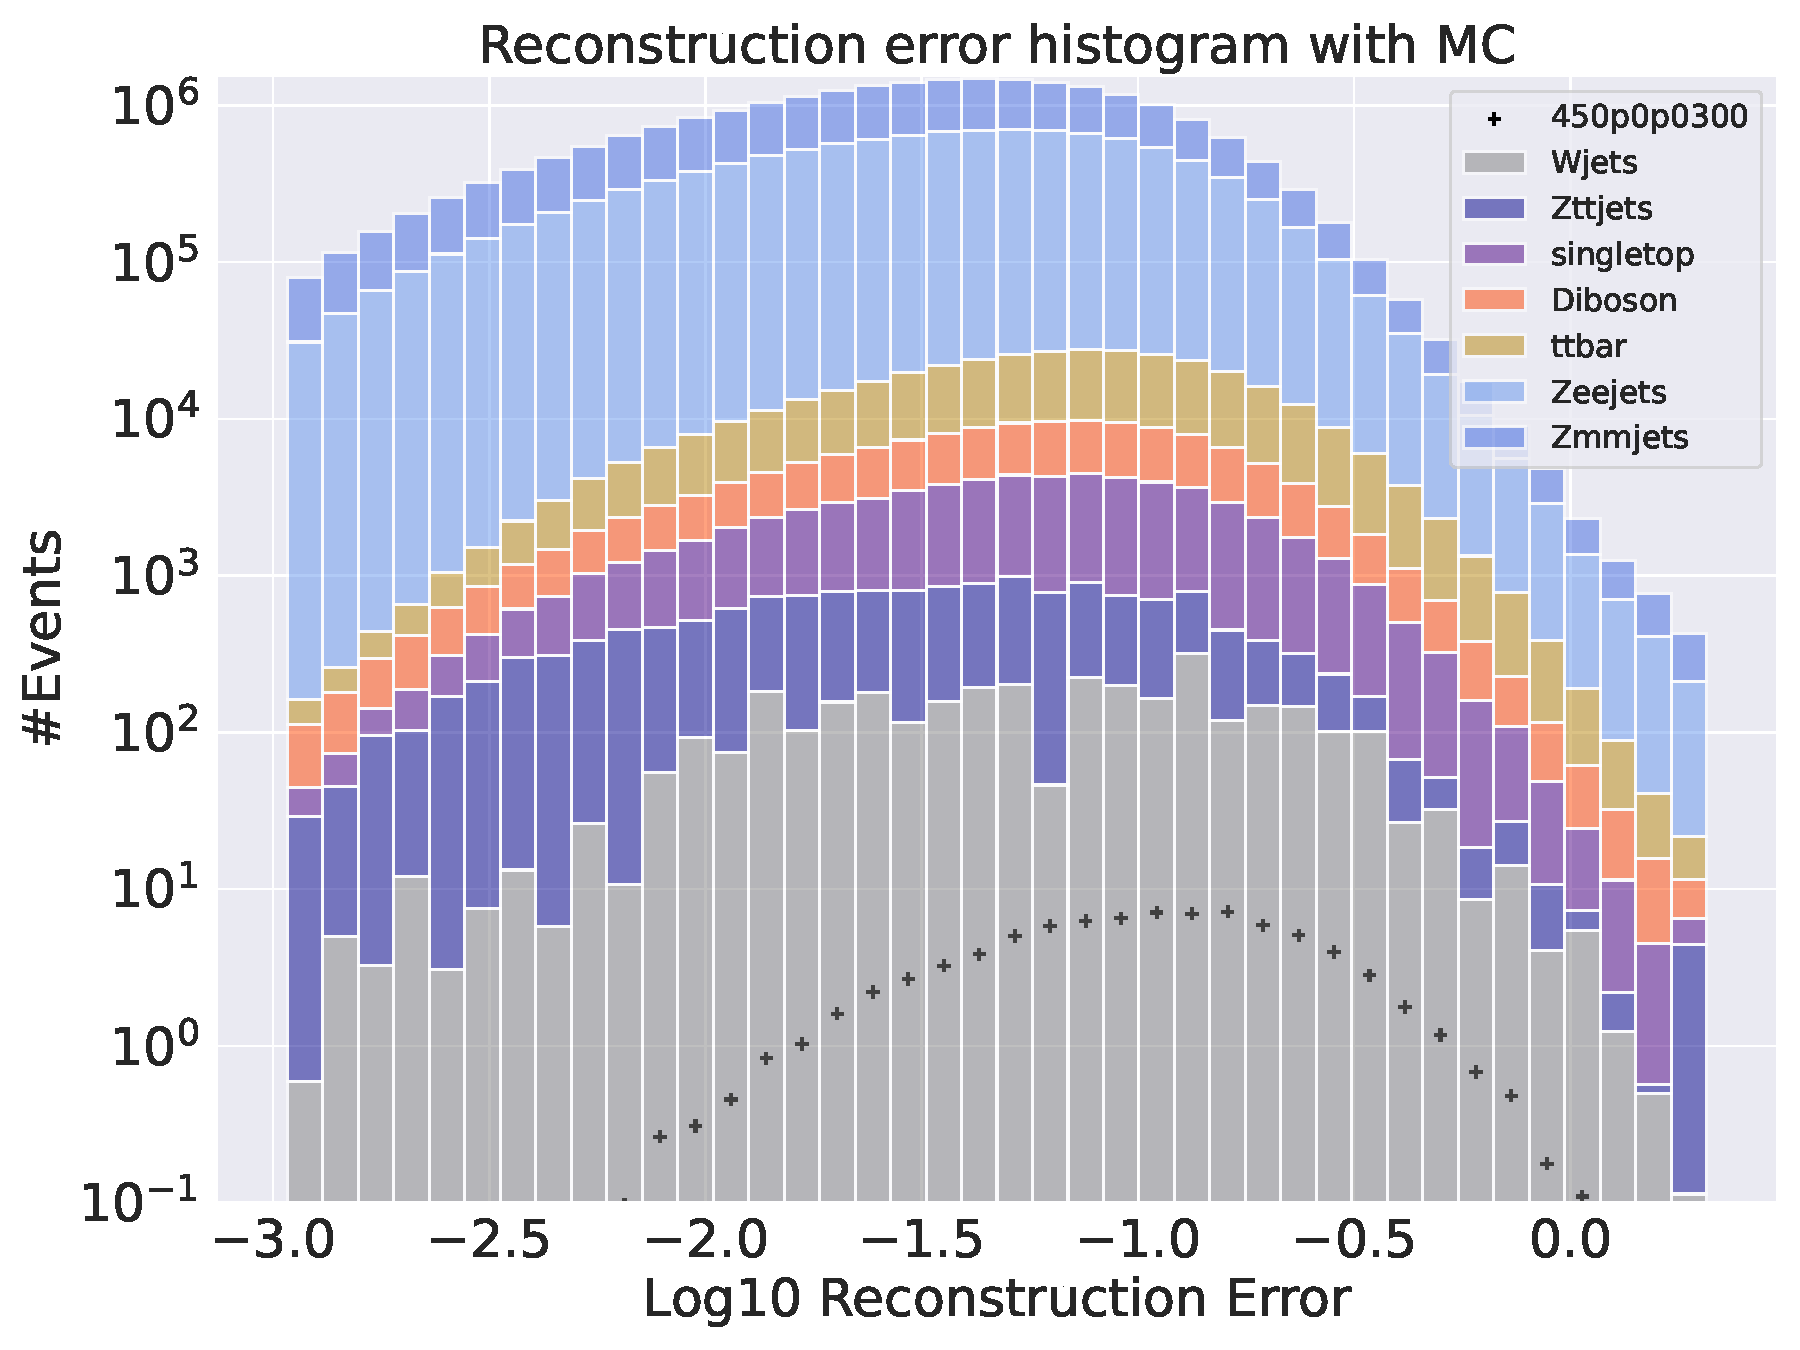
\includegraphics[width=\textwidth]{Figures/VAE_testing/small/2lep/b_data_recon_big_rm3_feats_sig_450p0p0300_.pdf}
        \caption{ }
        \label{fig:VAE_2lep_big_450}
    \end{subfigure}
    \hfill
    \begin{subfigure}{.60\textwidth}
        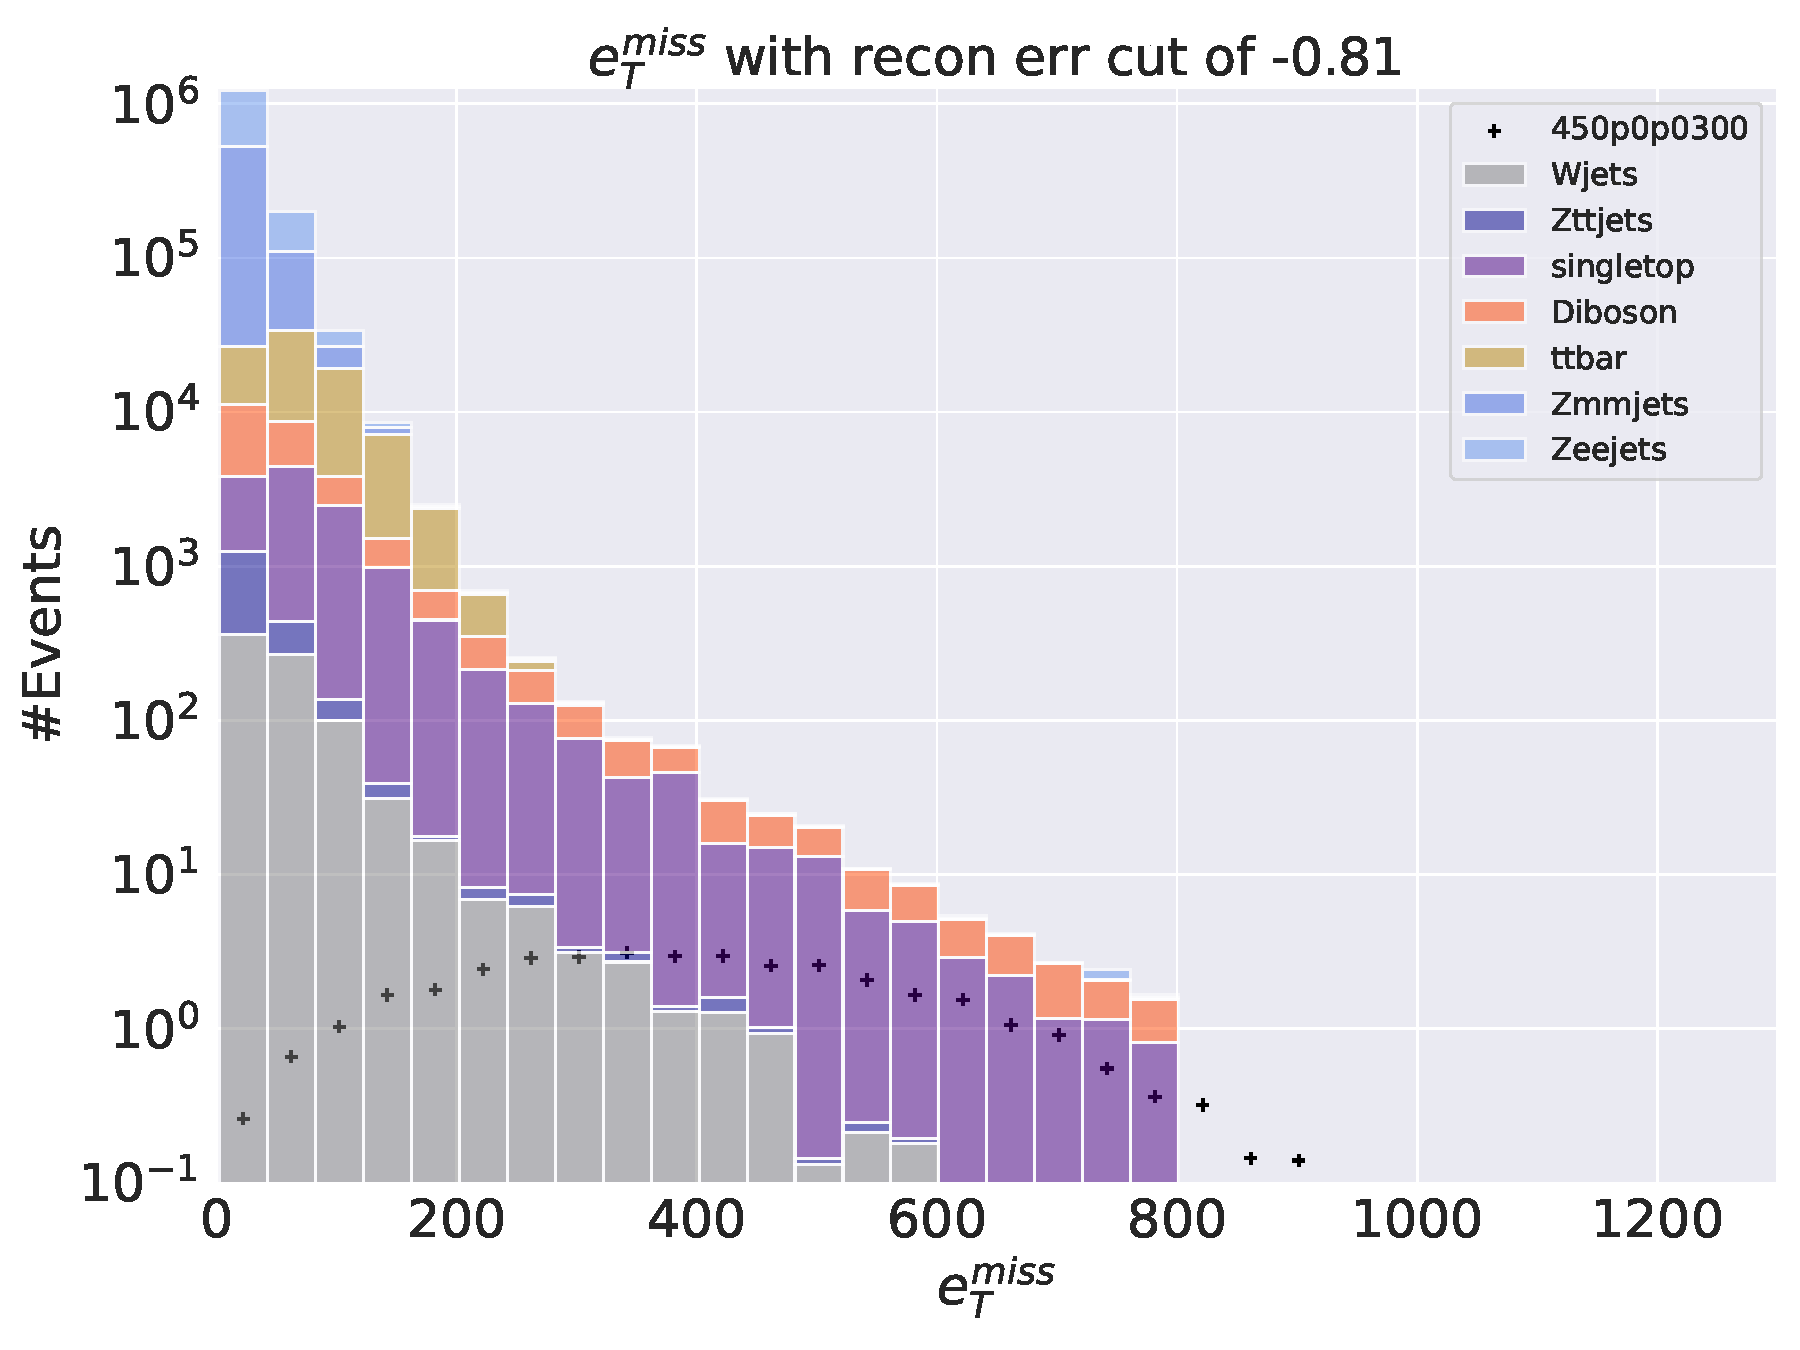
\includegraphics[width=\textwidth]{Figures/VAE_testing/big/2lep/b_data_recon_big_rm3_feats_sig_450p0p0300_recon_errcut_-0.81.pdf}
        \caption{}
        \label{fig:VAE_2lep_big_etmiss_450}
    \end{subfigure}
    \hfill 
    \begin{subfigure}{.60\textwidth}
        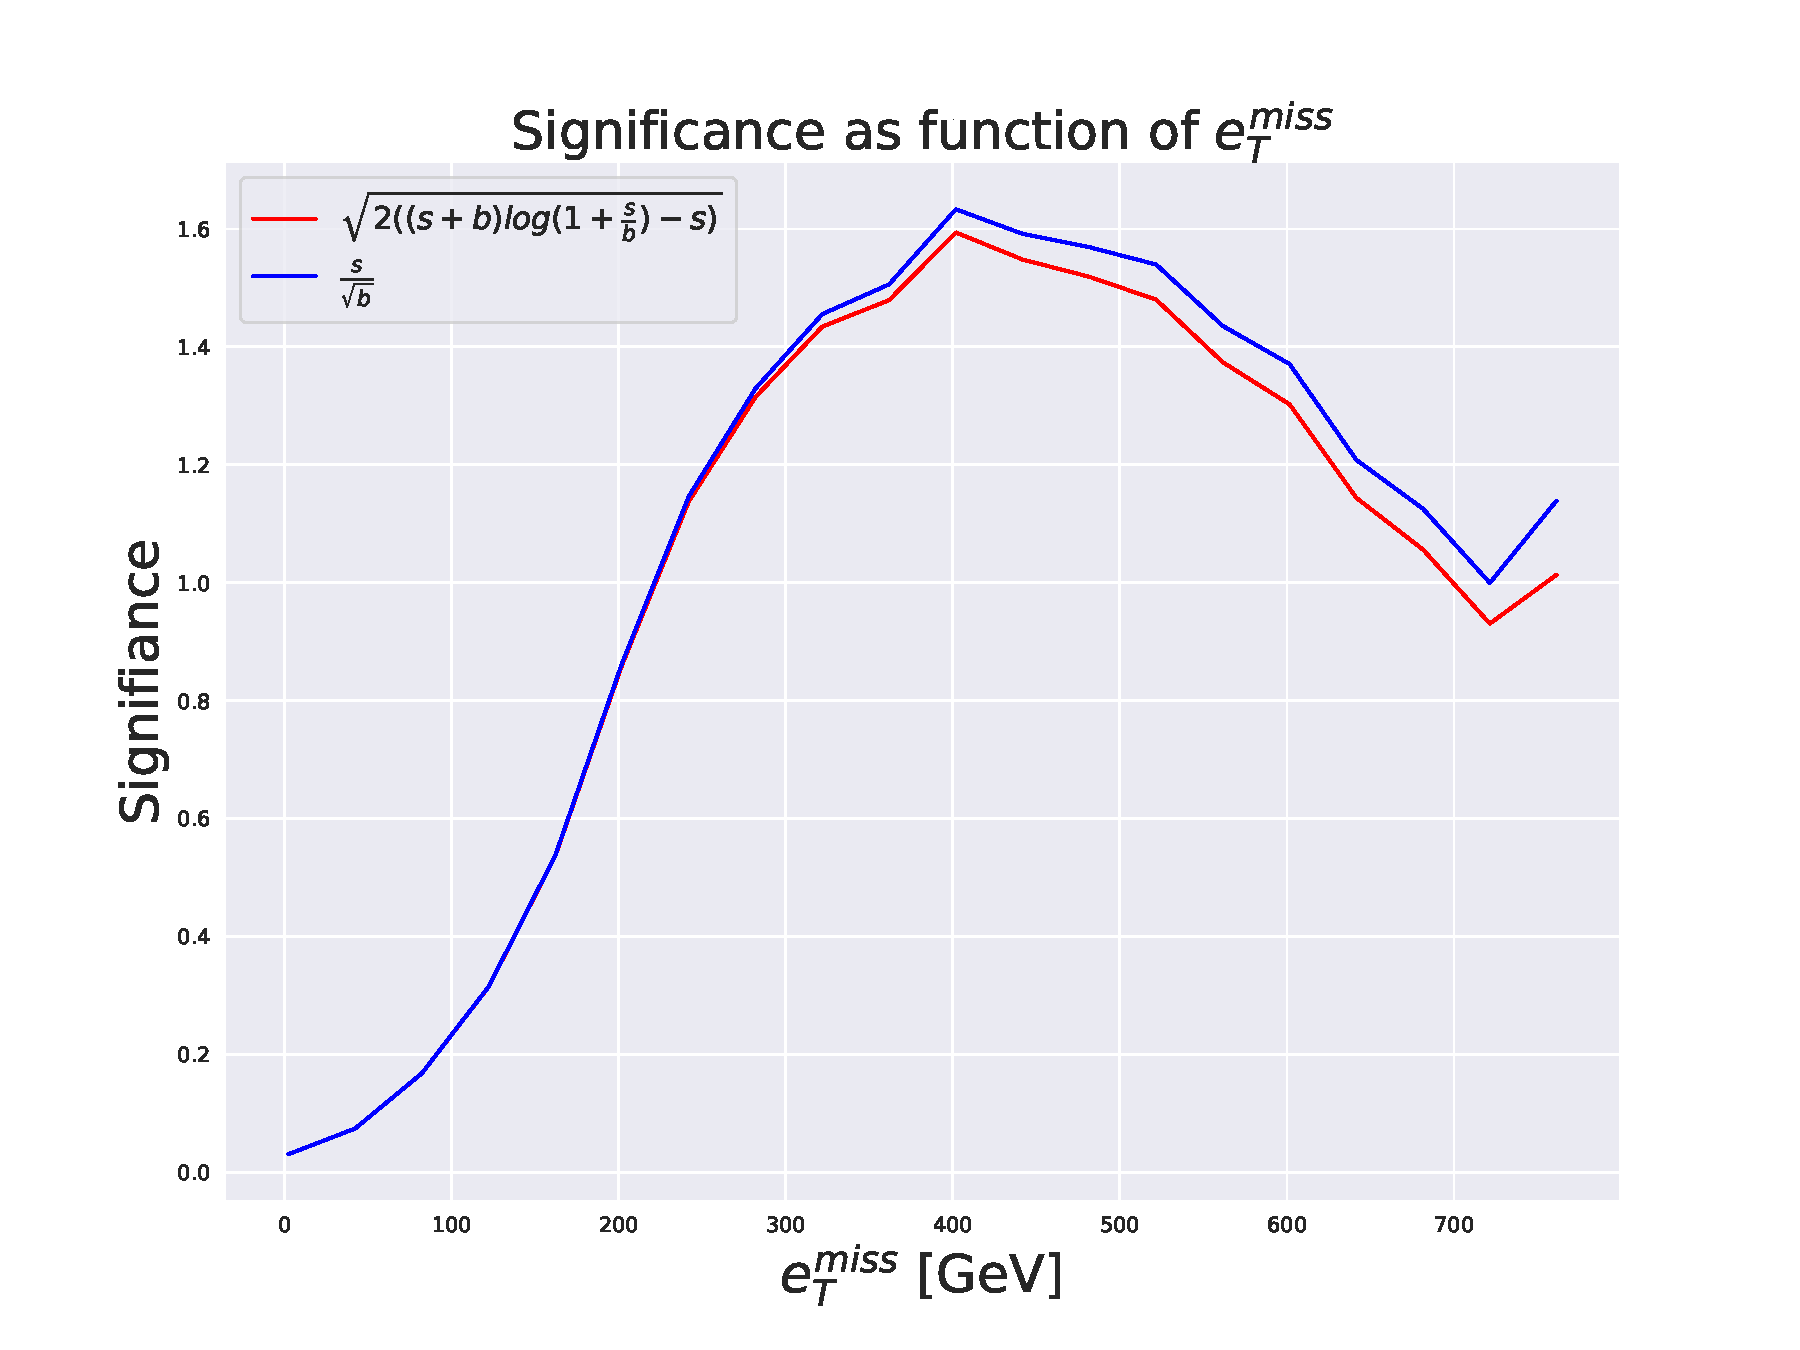
\includegraphics[width=\textwidth]{Figures/VAE_testing/big/2lep/significance_etmiss_450p0p0300_-0.8121874101107931.pdf}
        \caption{}
        \label{fig:VAE_2lep_big_signi_450}
    \end{subfigure}
    \hfill      
    \caption[2lep deep network | $450p300$ | VAE]{Reconstruction error, $e_T^{miss}$ signal region, $m_{lll}$ signal region and significance as function of 
    $e_T^{miss}$ for the deep regular autoencoder using SUSY $450p300$.}
    \label{fig:VAE_2lep_big_rec_sig_signi_450}
\end{figure}

\begin{figure}[H]
    \centering
    \begin{subfigure}{.60\textwidth}
        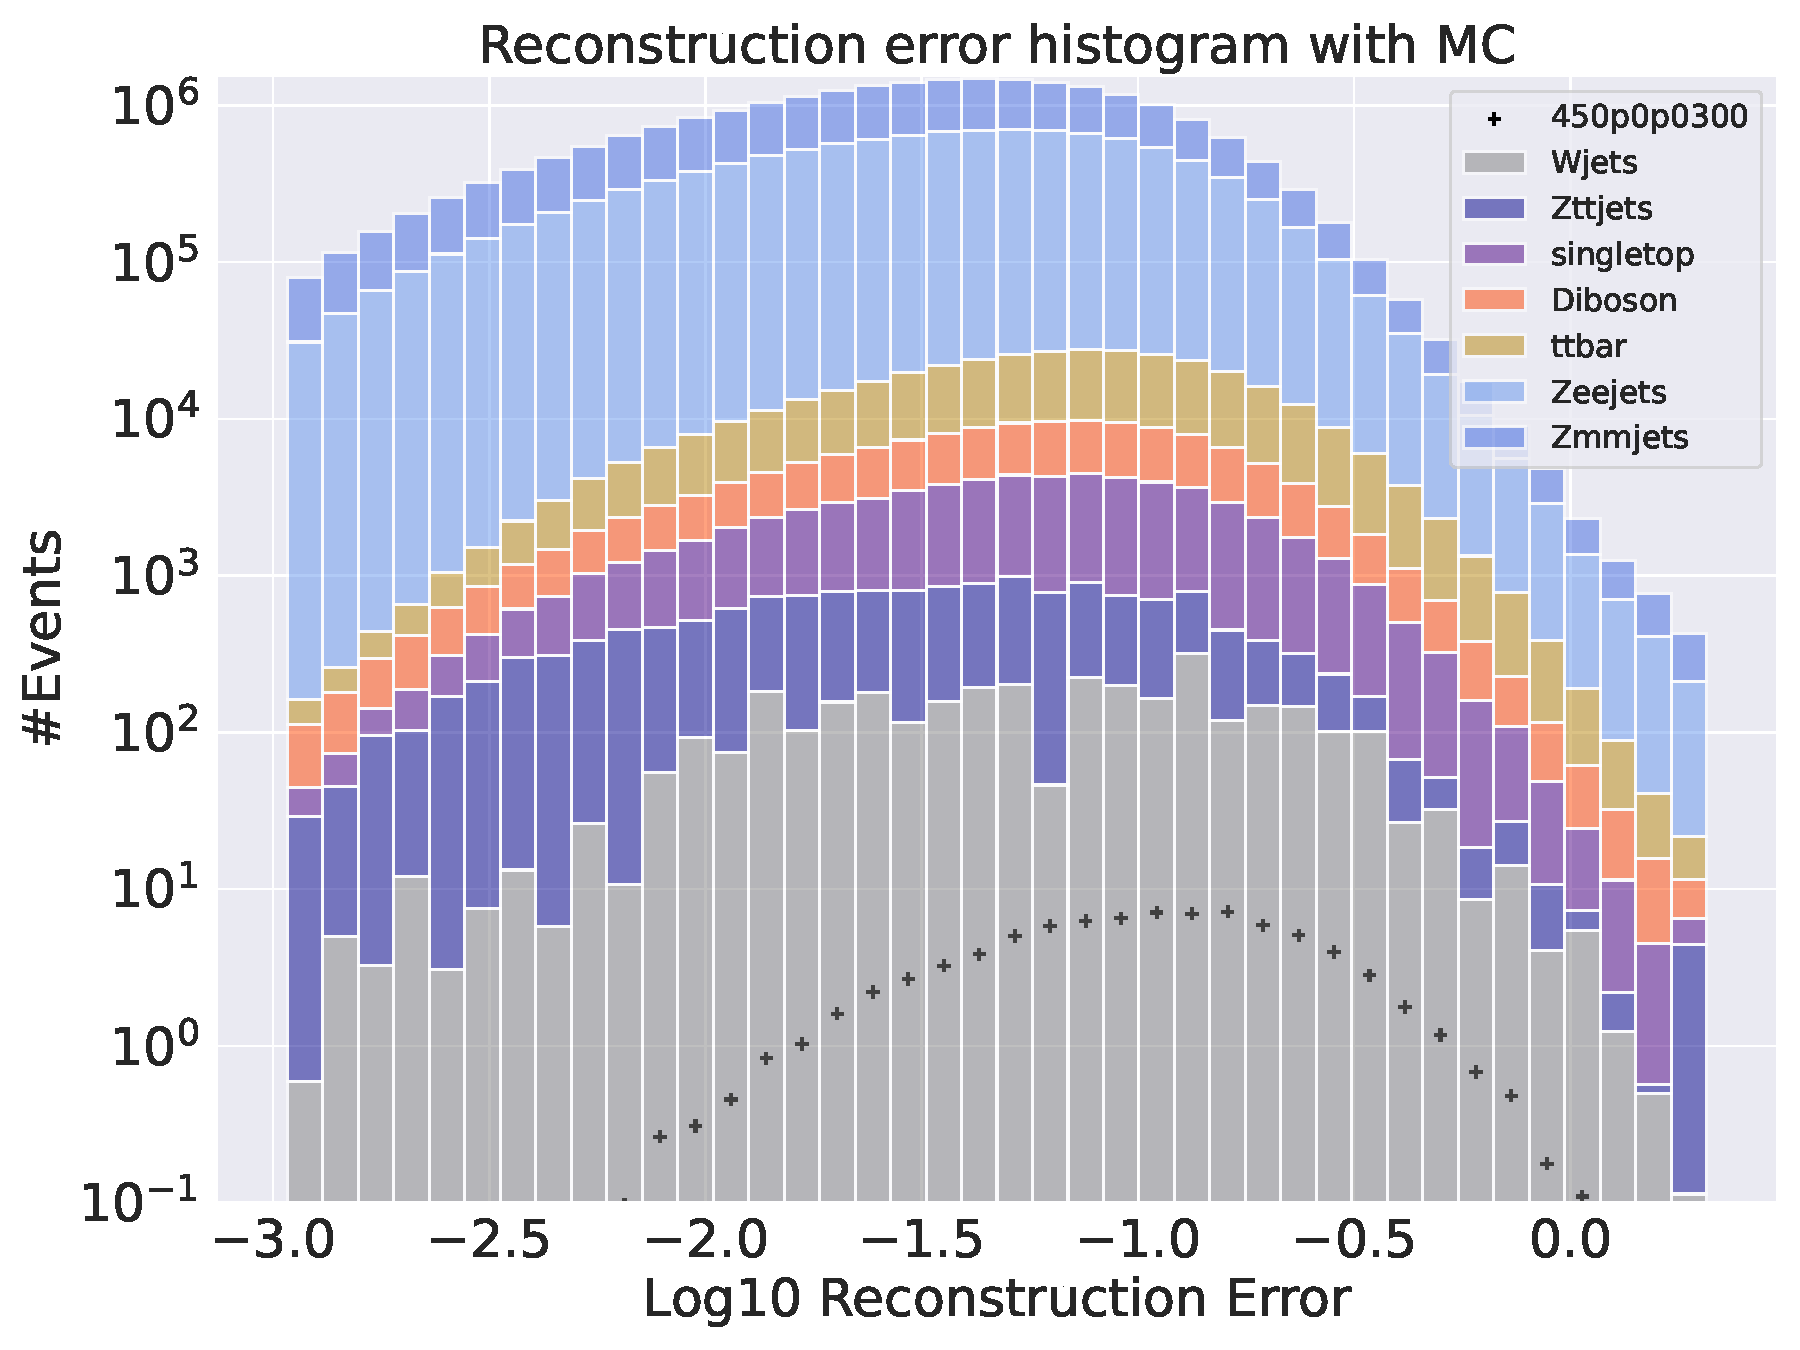
\includegraphics[width=\textwidth]{Figures/VAE_testing/small/2lep/b_data_recon_big_rm3_feats_sig_450p0p0300_.pdf}
        \caption{ }
        \label{fig:VAE_2lep_small_450}
    \end{subfigure}
    \hfill
    \begin{subfigure}{.60\textwidth}
        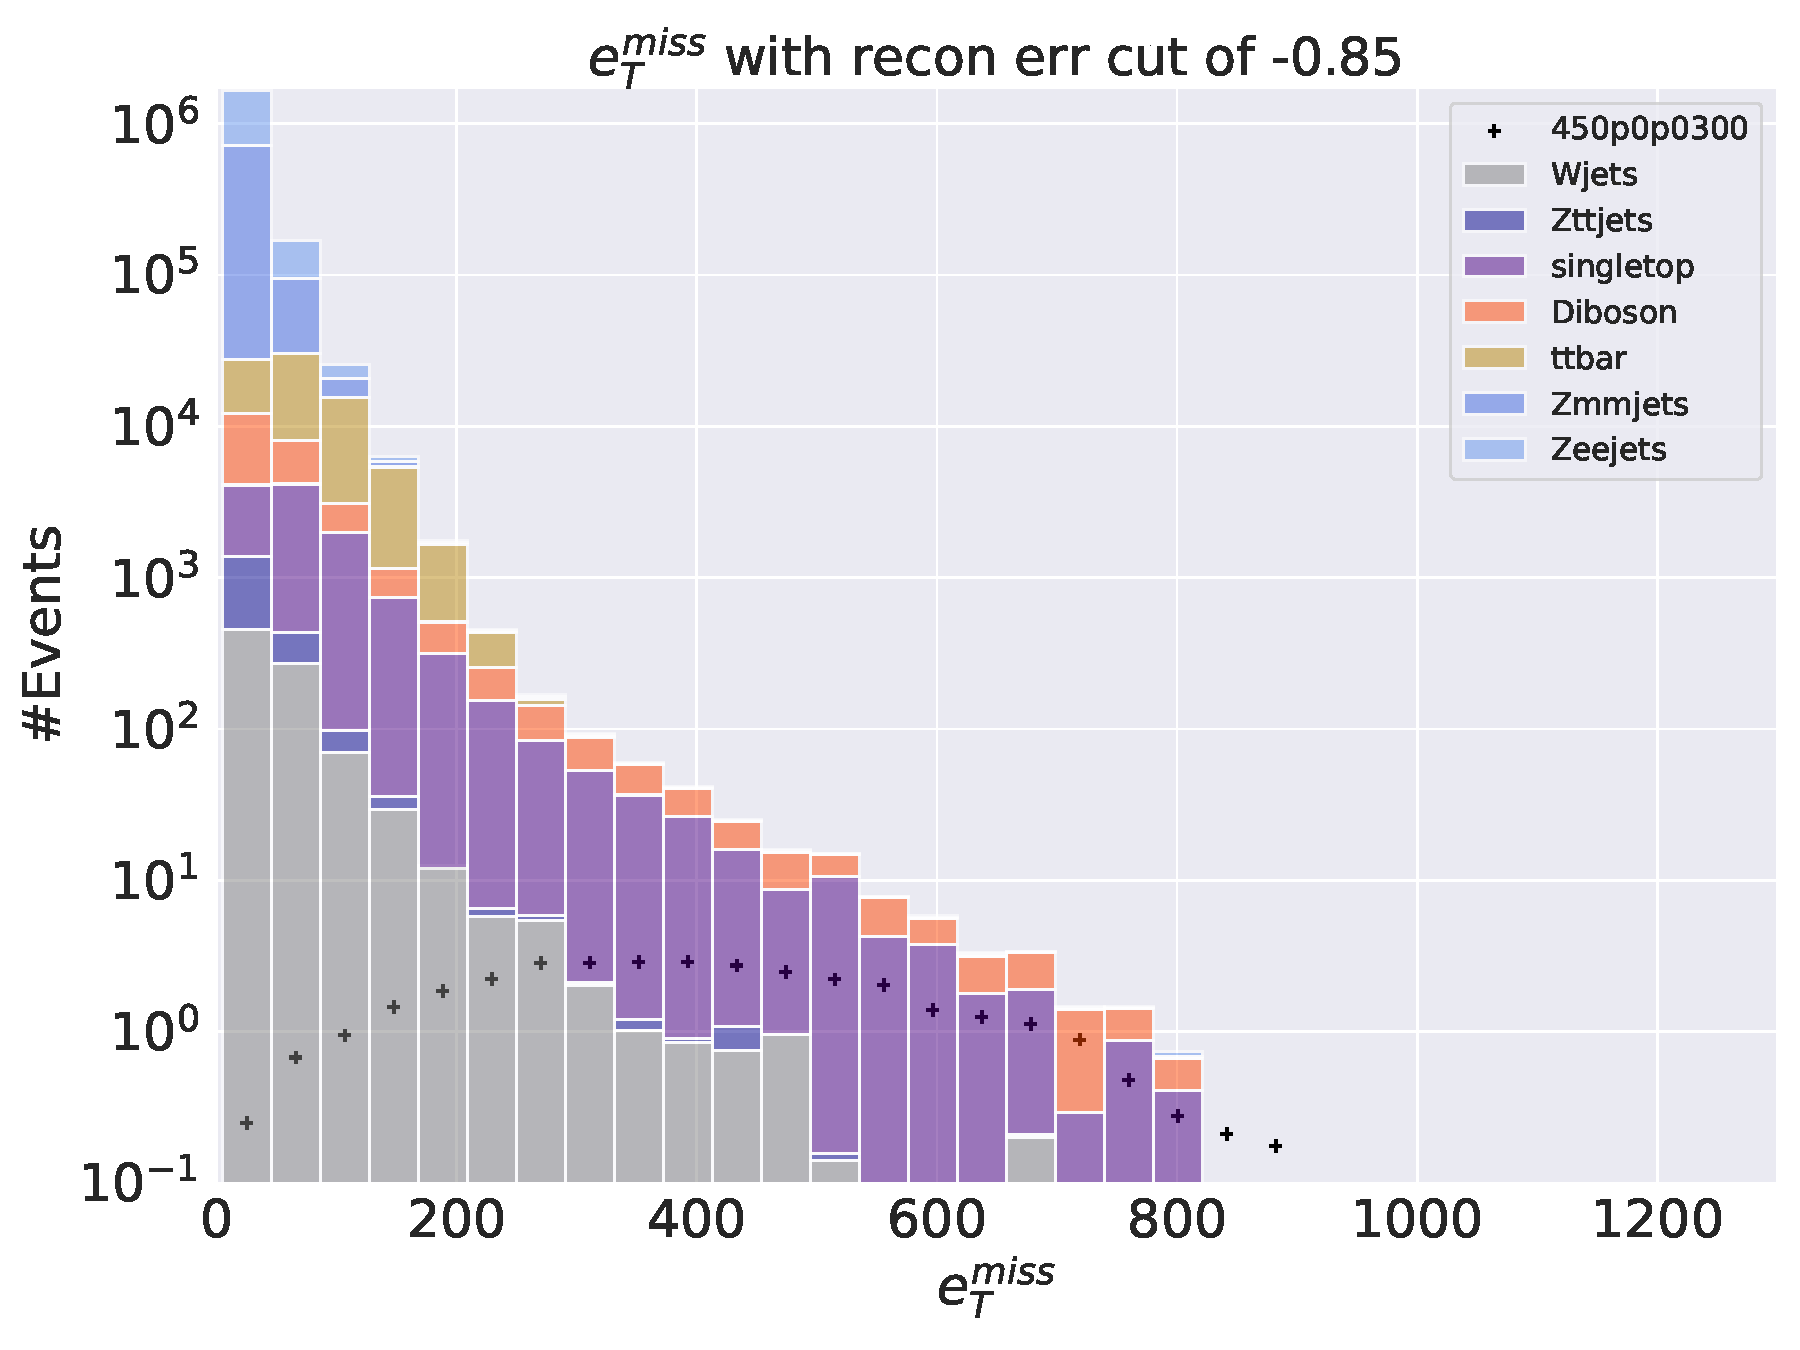
\includegraphics[width=\textwidth]{Figures/VAE_testing/small/2lep/b_data_recon_big_rm3_feats_sig_450p0p0300_recon_errcut_-0.85.pdf}
        \caption{}
        \label{fig:VAE_2lep_small_etmiss_450}
    \end{subfigure}
    \hfill  
    \begin{subfigure}{.60\textwidth}
        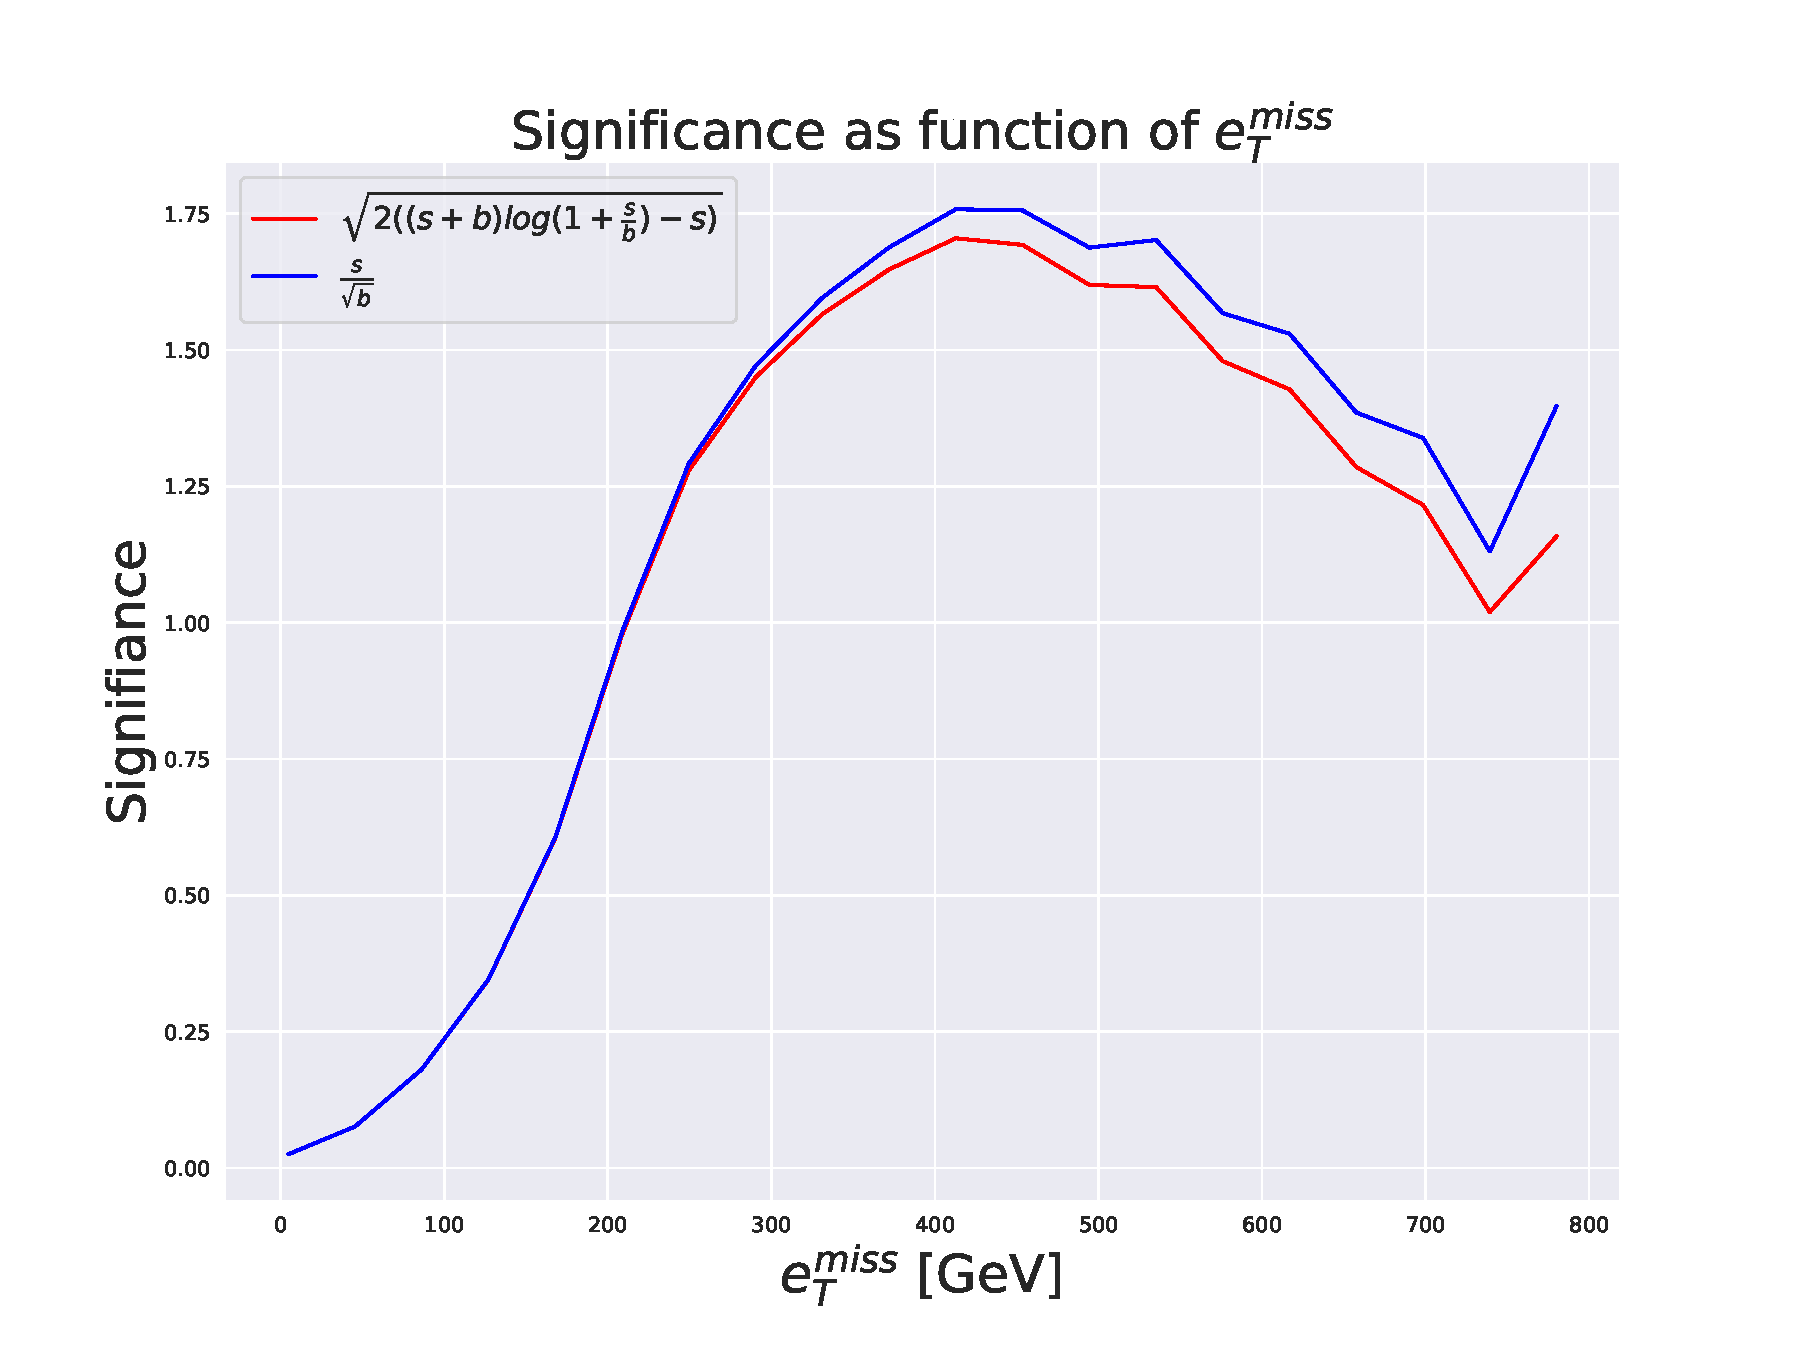
\includegraphics[width=\textwidth]{Figures/VAE_testing/small/2lep/significance_etmiss_450p0p0300_-0.8484803499636524.pdf}
        \caption{}
        \label{fig:VAE_2lep_small_signi_450}
    \end{subfigure}
    \hfill      
    \caption[2lep shallow network | $450p300$ | VAE]{Reconstruction error, $e_T^{miss}$ signal region, $m_{lll}$ signal region and significance as function of 
    $e_T^{miss}$ for the shallow regular autoencoder using SUSY $450p300$.}
    \label{fig:VAE_2lep_small_rec_sig_signi_450}
\end{figure}


\begin{figure}[H]
    \centering
    \begin{subfigure}{.60\textwidth}
        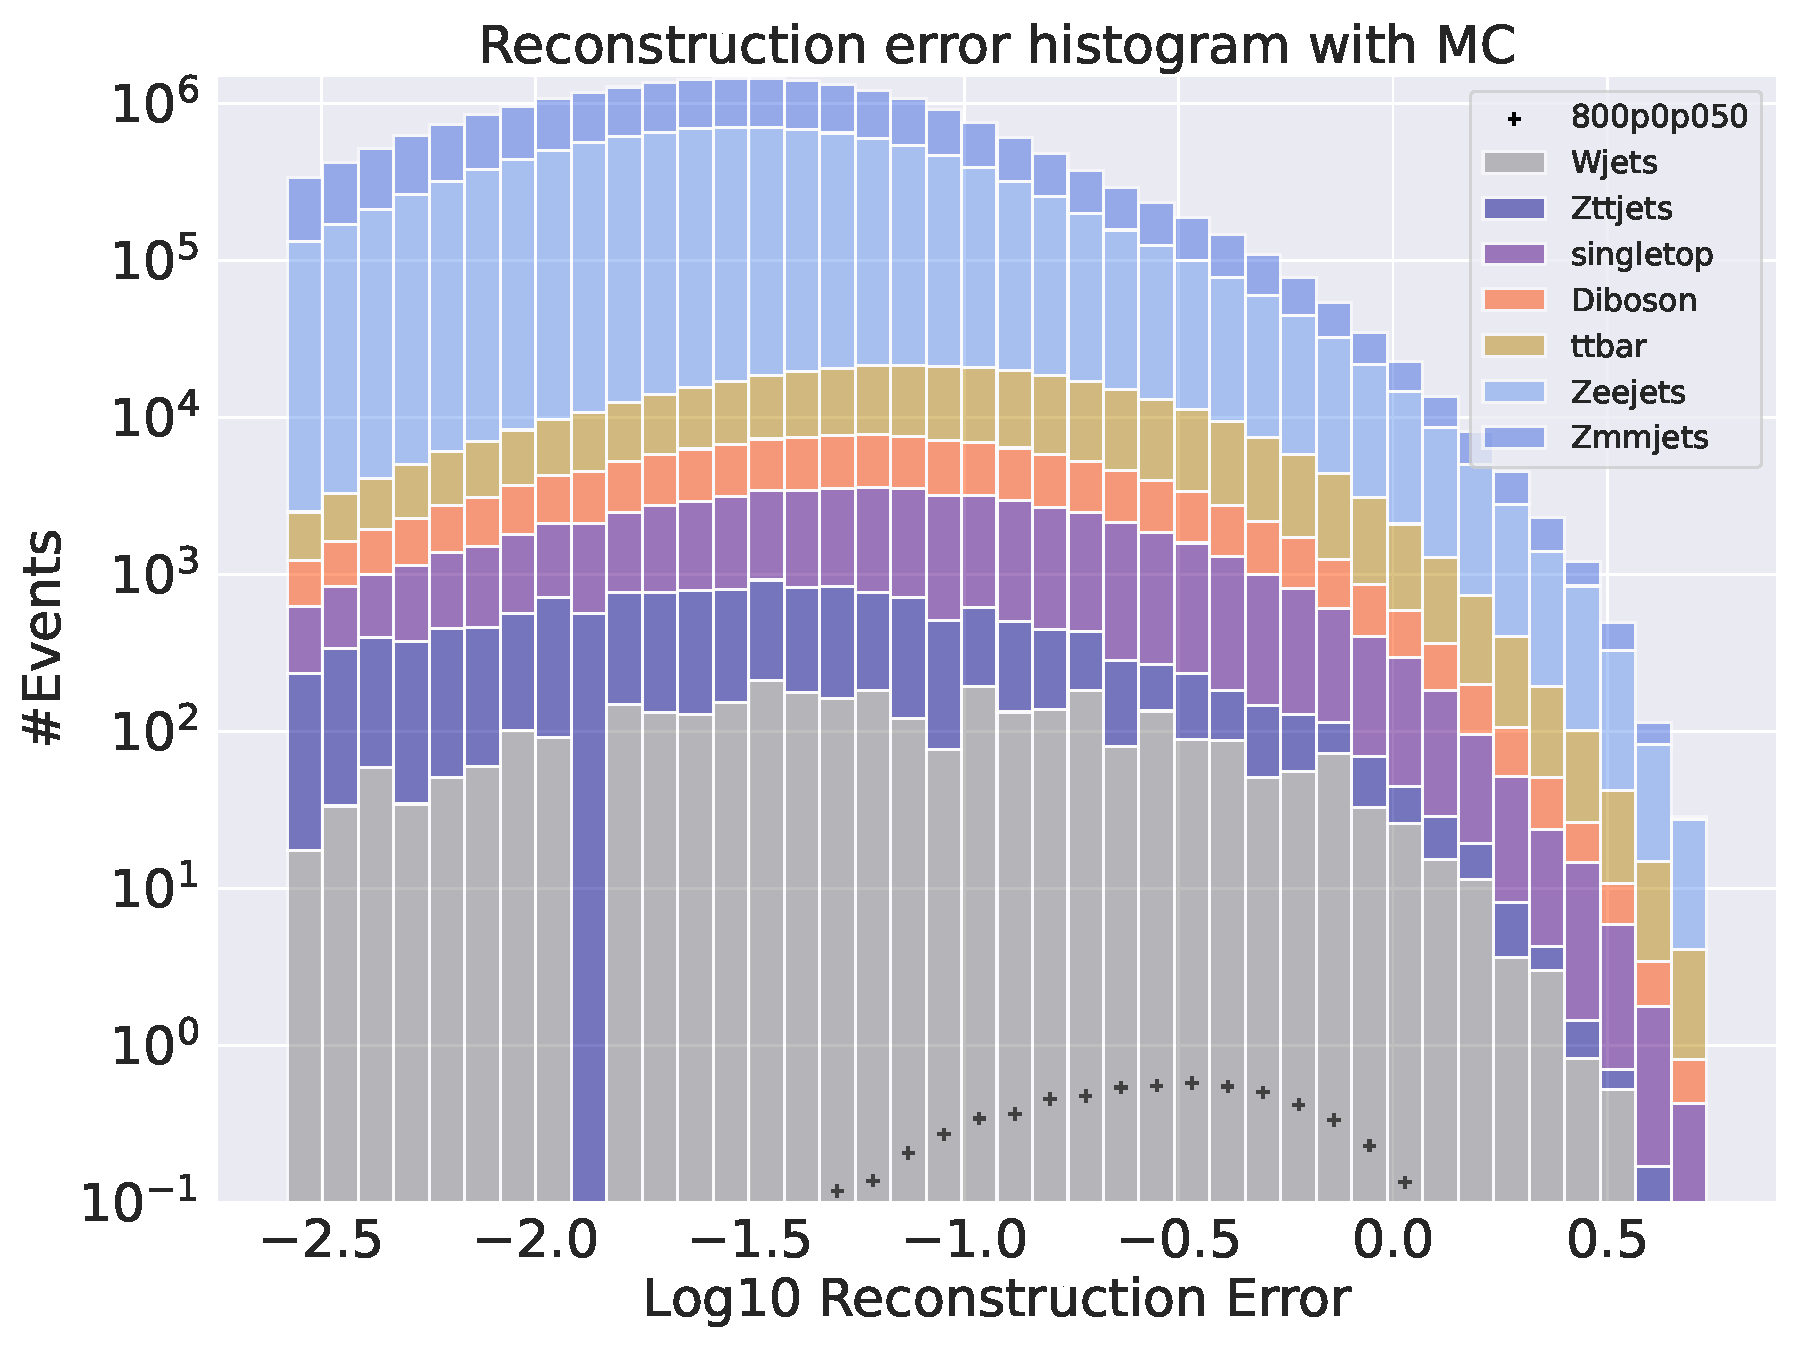
\includegraphics[width=\textwidth]{Figures/VAE_testing/big/2lep/b_data_recon_big_rm3_feats_sig_800p0p050_.pdf}
        \caption{ }
        \label{fig:VAE_2lep_big_800}
    \end{subfigure}
    \hfill
    \begin{subfigure}{.60\textwidth}
        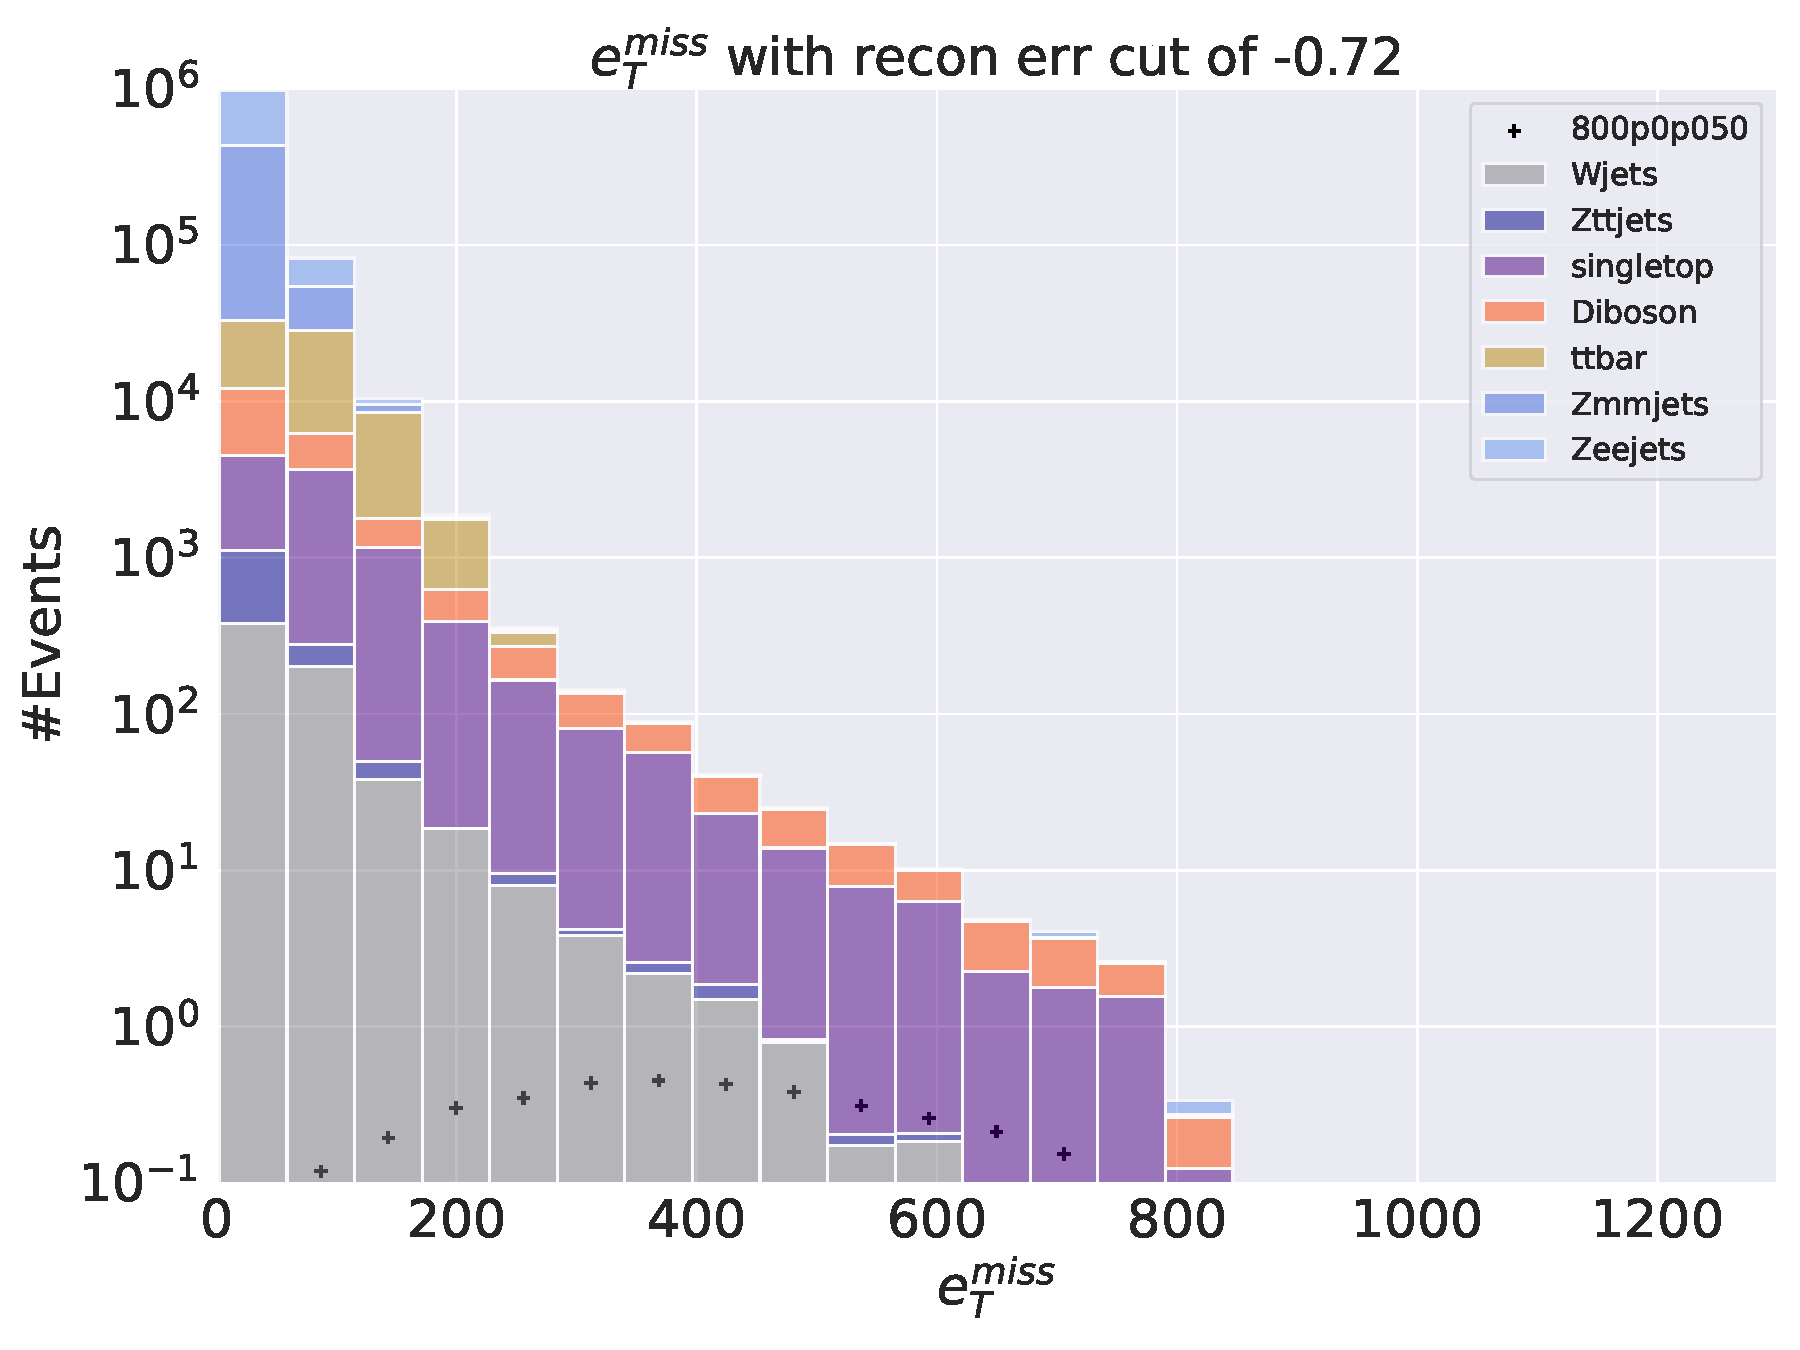
\includegraphics[width=\textwidth]{Figures/VAE_testing/big/2lep/b_data_recon_big_rm3_feats_sig_800p0p050_recon_errcut_-0.72.pdf}
        \caption{}
        \label{fig:VAE_2lep_big_etmiss_800}
    \end{subfigure}
    \hfill
      
    \begin{subfigure}{.60\textwidth}
        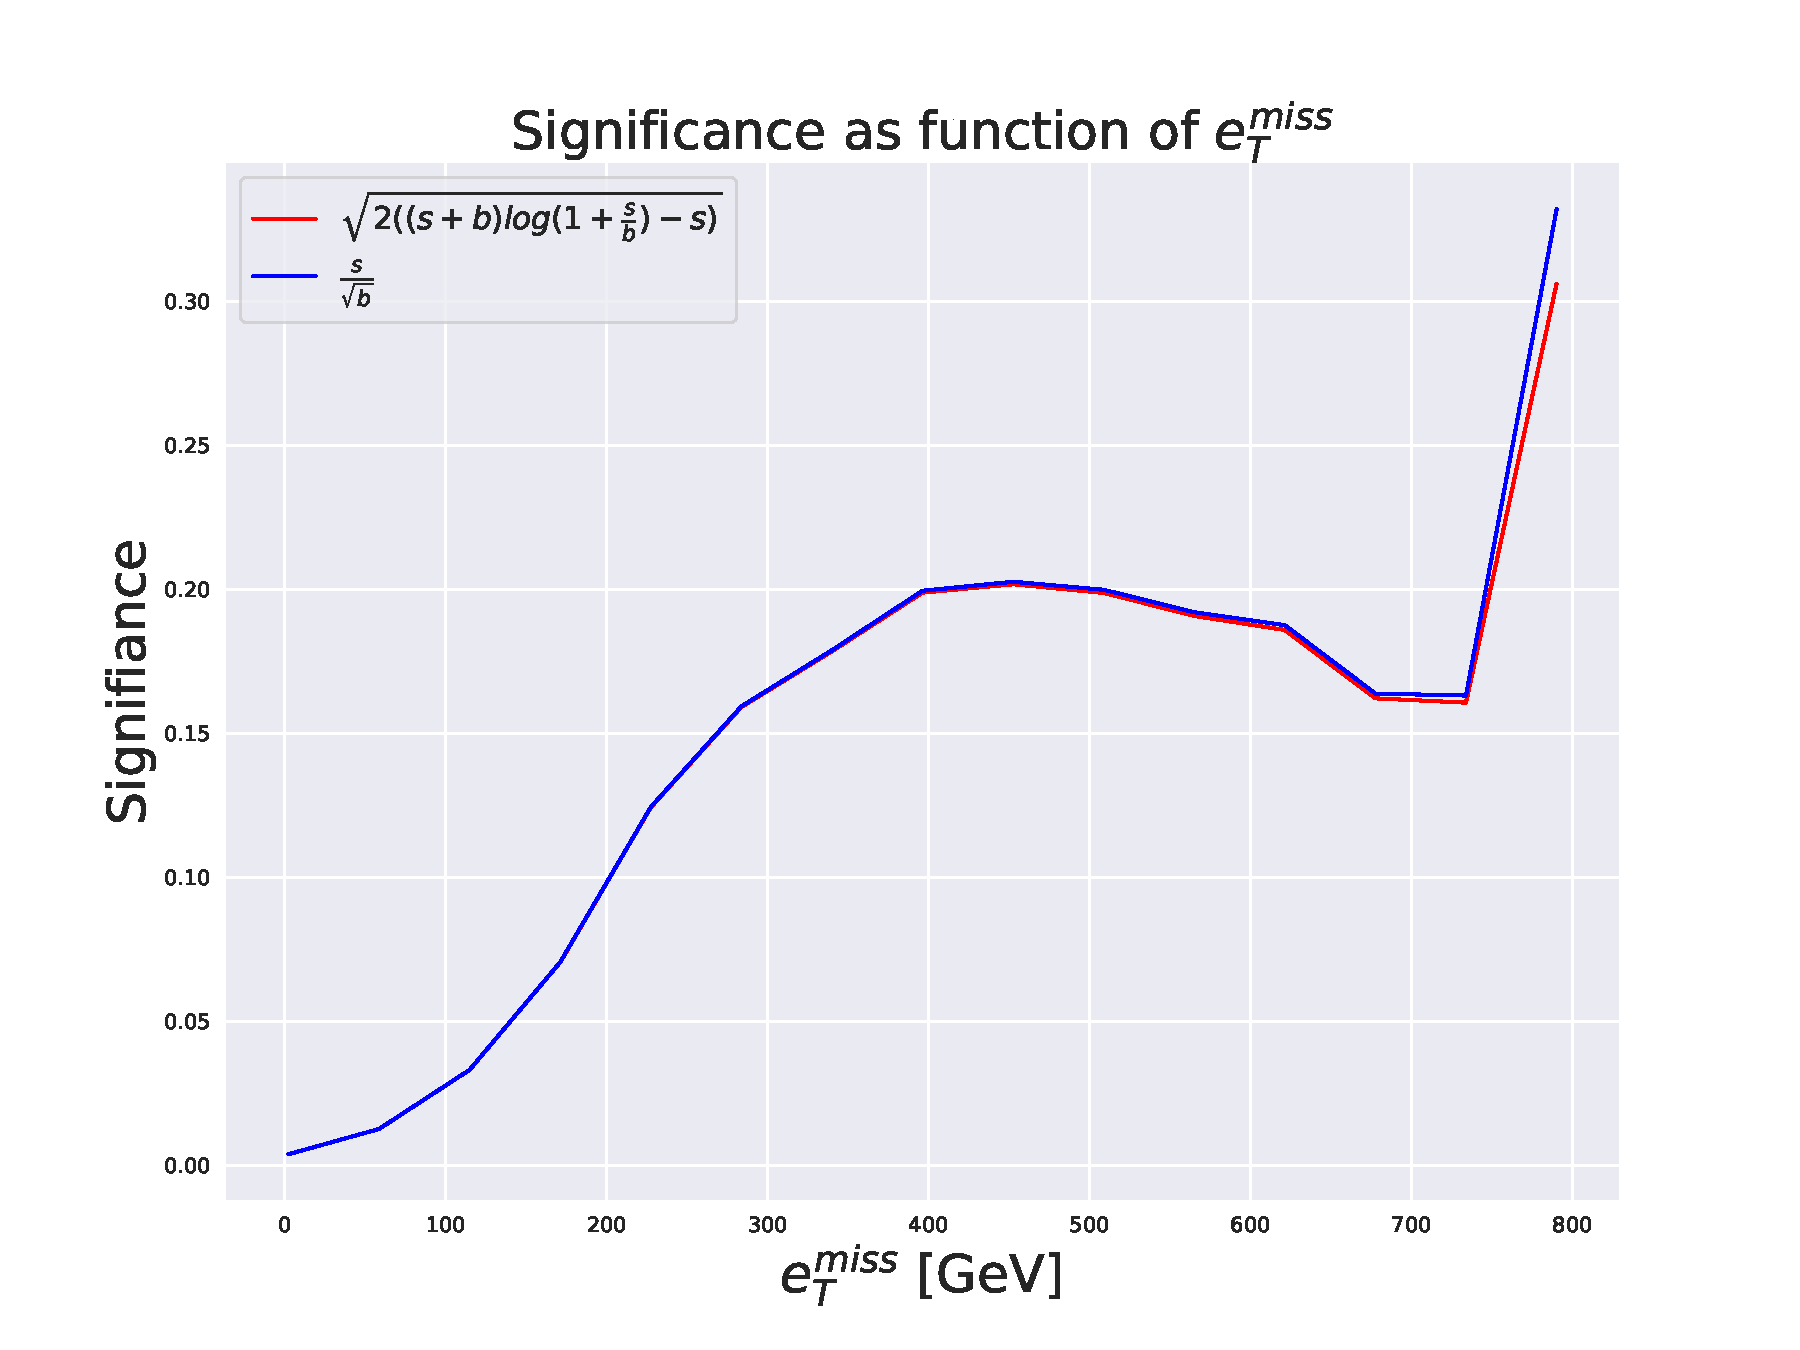
\includegraphics[width=\textwidth]{Figures/VAE_testing/big/2lep/significance_etmiss_800p0p050_-0.7232197345309495.pdf}
        \caption{}
        \label{fig:VAE_2lep_big_signi_800}
    \end{subfigure}
    \hfill      
    \caption[2lep deep network | $800p50$ | VAE]{Reconstruction error, $e_T^{miss}$ signal region, $m_{lll}$ signal region and significance as function of 
    $e_T^{miss}$ for the deep variational autoencoder using SUSY $800p50$.}
    \label{fig:VAE_2lep_big_rec_sig_signi_800}
\end{figure}

\begin{figure}[H]
    \centering
    \begin{subfigure}{.60\textwidth}
        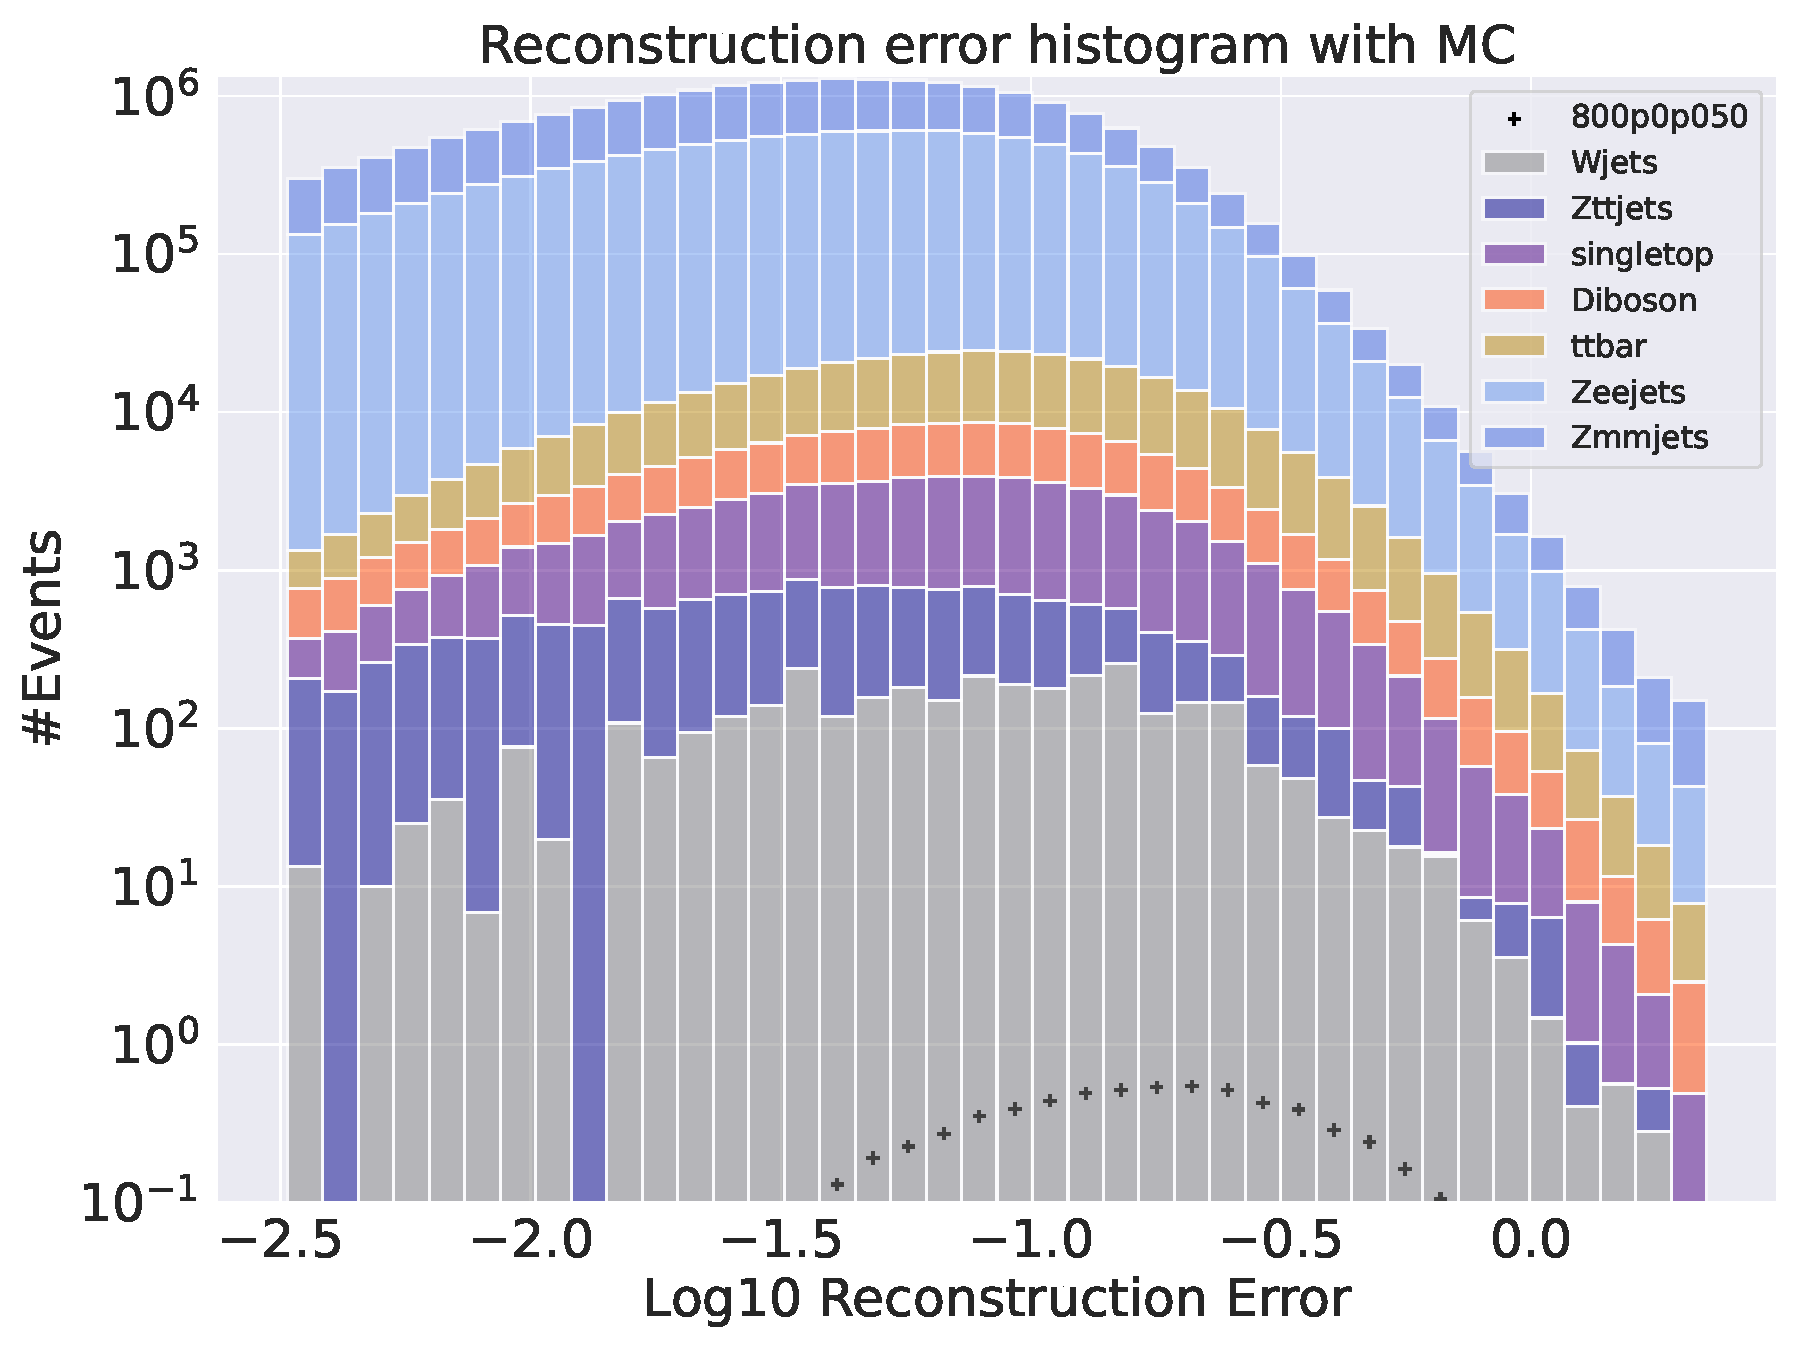
\includegraphics[width=\textwidth]{Figures/VAE_testing/small/2lep/b_data_recon_big_rm3_feats_sig_800p0p050_.pdf}
        \caption{ }
        \label{fig:VAE_2lep_small_800}
    \end{subfigure}
    \hfill
    \begin{subfigure}{.60\textwidth}
        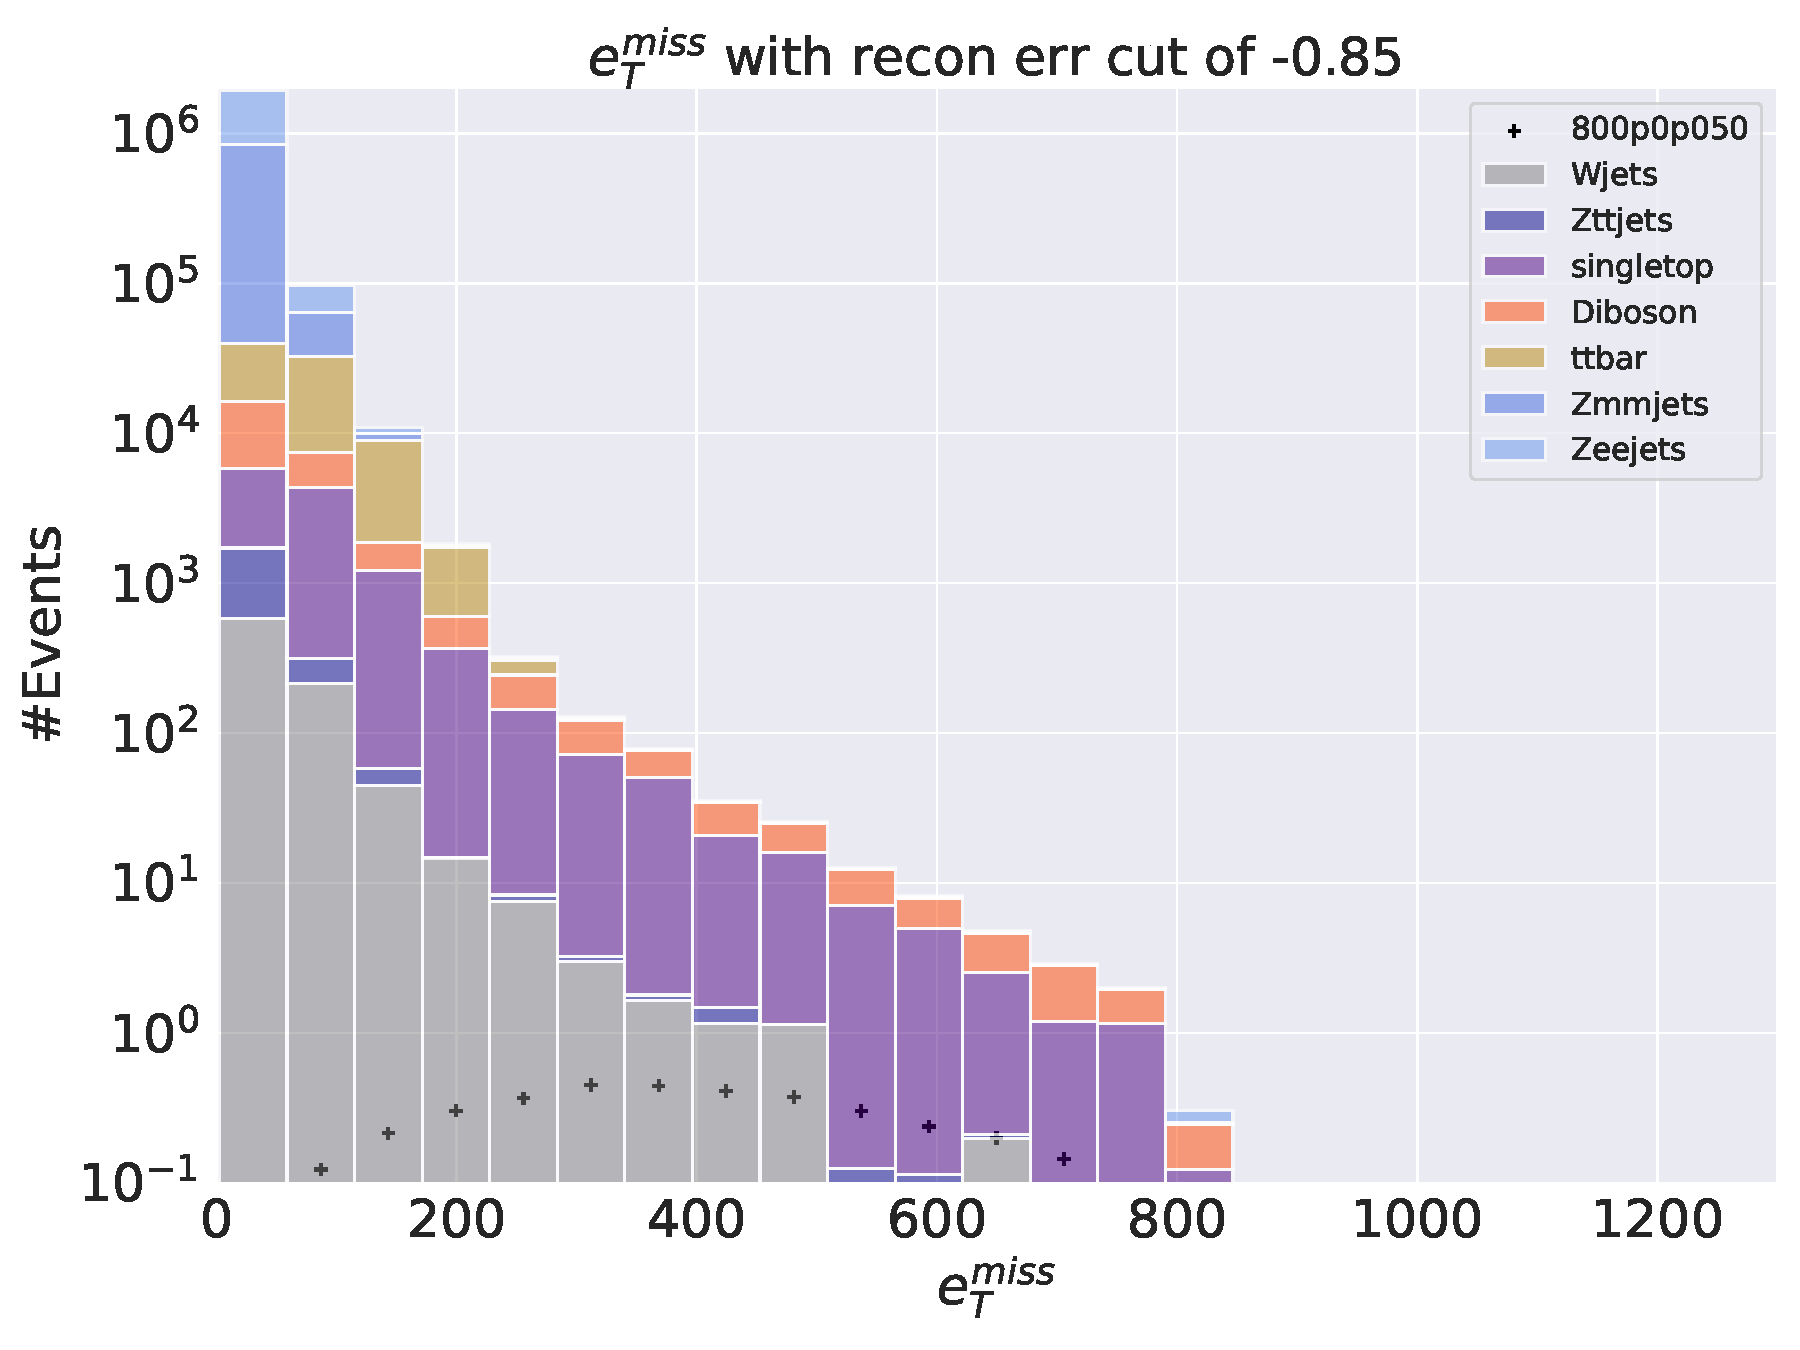
\includegraphics[width=\textwidth]{Figures/VAE_testing/small/2lep/b_data_recon_big_rm3_feats_sig_800p0p050_recon_errcut_-0.85.pdf}
        \caption{}
        \label{fig:VAE_2lep_small_etmiss_800}
    \end{subfigure}
    \hfill  
    \begin{subfigure}{.60\textwidth}
        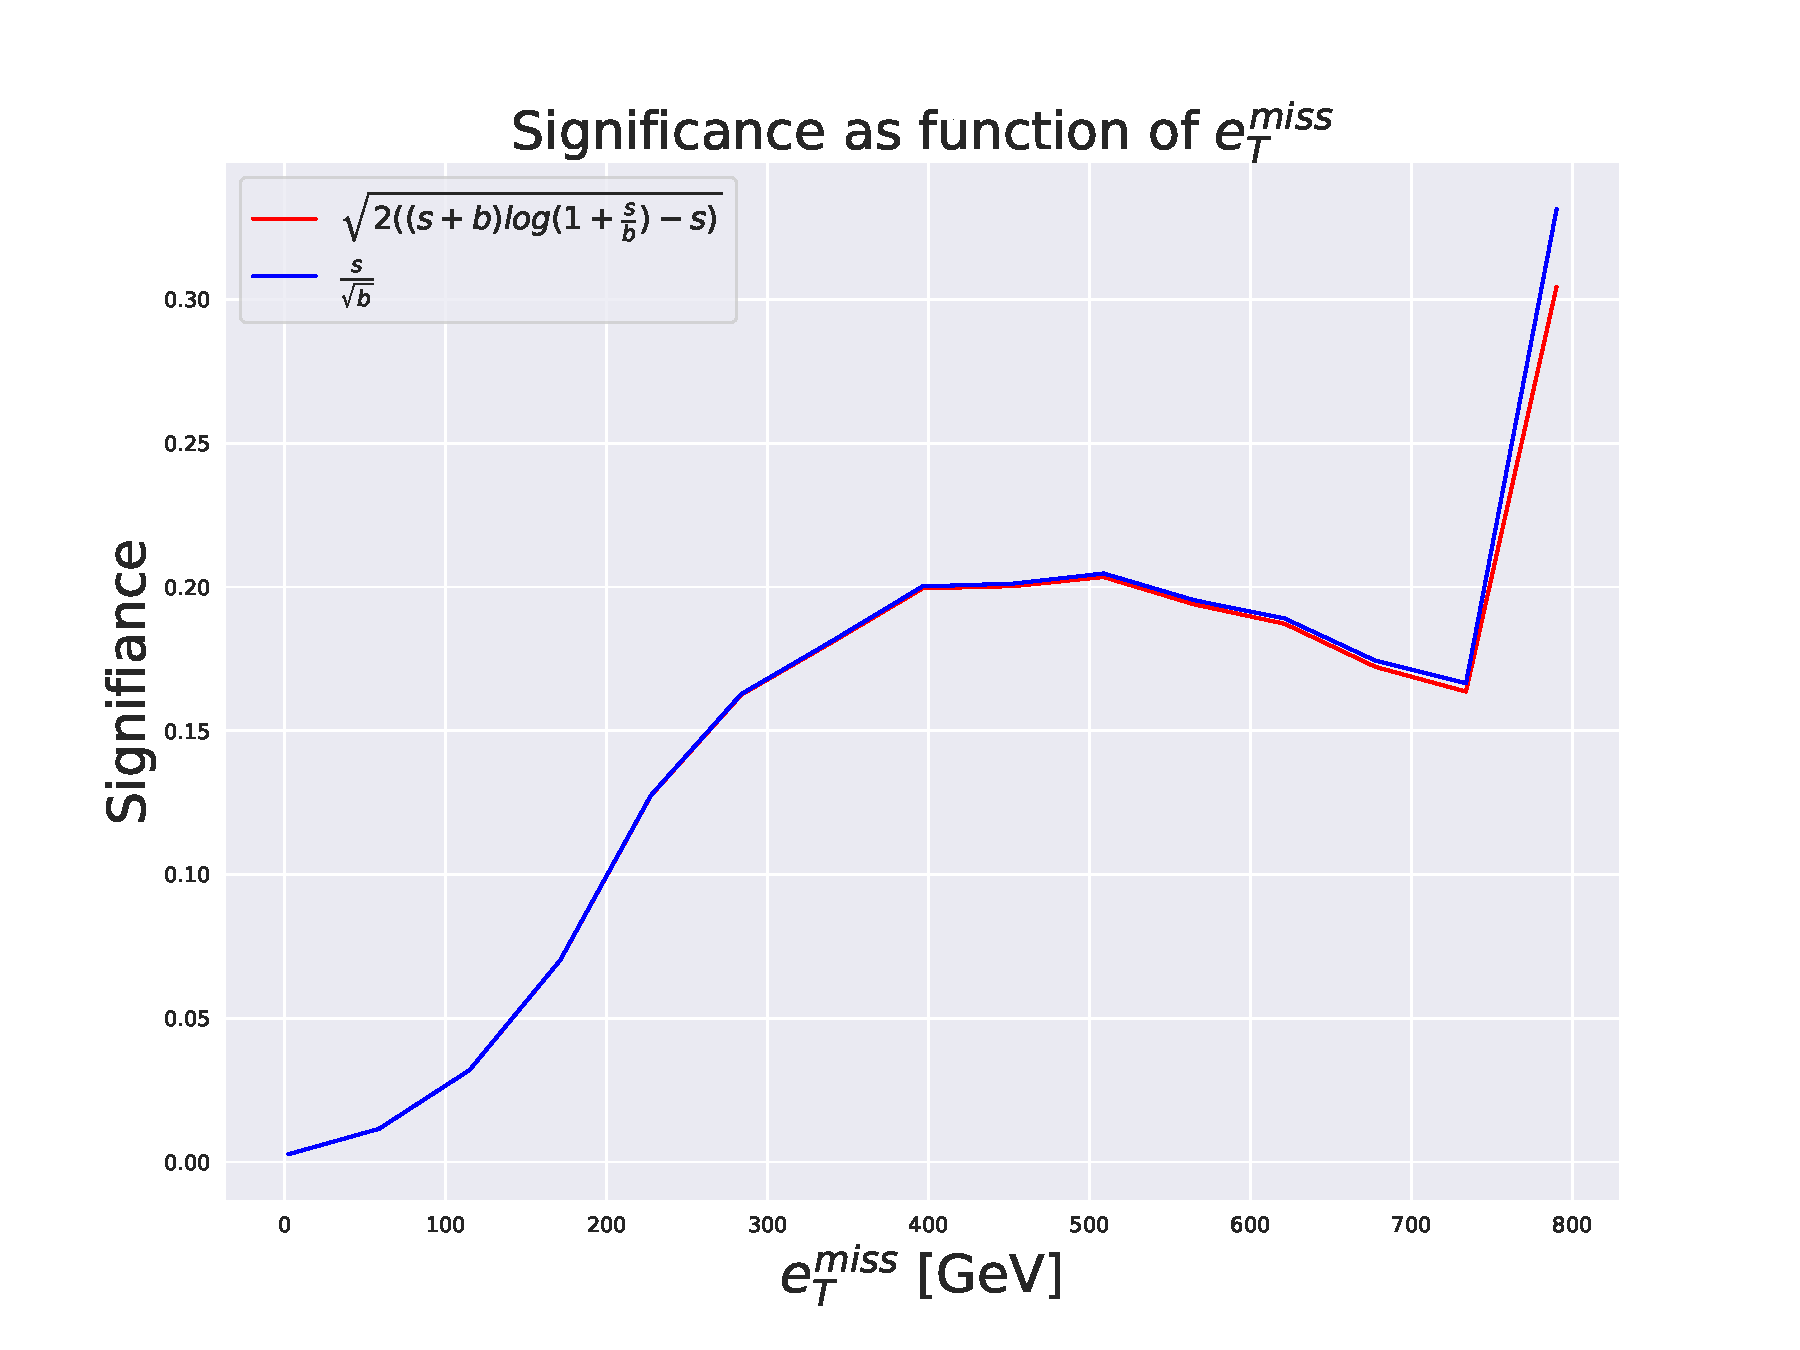
\includegraphics[width=\textwidth]{Figures/VAE_testing/small/2lep/significance_etmiss_800p0p050_-0.8542149600758421.pdf}
        \caption{}
        \label{ffig:VAE_2lep_small_signi_800}
    \end{subfigure}
    \hfill      
    \caption[2lep shallow network | $800p50$ | VAE]{Reconstruction error, $e_T^{miss}$ signal region, $m_{lll}$ signal region and significance as function of 
    $e_T^{miss}$ for the shallow variational autoencoder using SUSY $800p50$.}
    \label{fig:VAE_2lep_small_rec_sig_signi_800}
\end{figure}


In figures \ref{fig:VAE_2lep_big_rec_sig_signi_450}, \ref{fig:VAE_2lep_small_rec_sig_signi_450}, 
\ref{fig:VAE_2lep_big_rec_sig_signi_800} and \ref{fig:VAE_2lep_small_rec_sig_signi_800} we have three 
subplots containing the total reconstruction error distributions, the $e_T^{miss}$ signal region, 
and the significance as function of $e_T^{miss}$ curve respectively. They were created using 
the shallow and deep regular autoencoder with the 2 lepton + $e_T^{miss}$ dataset.
In figures \ref{fig:VAE_2lep_big_450}, \ref{fig:VAE_2lep_small_450}, \ref{fig:VAE_2lep_big_800}, 
\ref{fig:VAE_2lep_small_800} we have the reconstruction error distributions 
for both SUSY signals for the small and large variational autoencoder. Here we observe that the 
peak of the distributions for the SM MC in all four cases are somewhat centered in the middle 
of the reconstruction error range, which differs from the steep slope we saw in figures 
\ref{fig:AE_2lep_big_450}, \ref{fig:AE_2lep_small_450}, \ref{fig:AE_2lep_big_800}, 
\ref{fig:AE_2lep_small_800}. Interestingly, we see here that the deepness of the neural 
network here plays a role, which is different from the regular autoencoder output, where both 
the small and large autoencoder made a steep slope shape of the SM MC reconstruction error 
distribution. The peak of the distribution here is slightly shifted to the left for the shallow 
autoencoder model, and slightly shifted to the right of the center with the deep autoencoder 
model. One possible reason for this somewhat Gaussian like distribution could be that the 
variational autoencoder, via the reparametization trick from section \ref{sec:reparameterization}, 
samples from a Gaussian distribution that has yet to be trained on enough data to produce a 
good enough error distribution. This is also supported with the fact that the shape is even more 
Gaussian like in the 3 lepton + $e_T^{miss}$ case shown in figures \ref{fig:VAE_3lep_big_450}, 
\ref{fig:VAE_3lep_small_450}, \ref{fig:VAE_3lep_big_800}, \ref{fig:VAE_3lep_small_800}. 
It could also be that the batch size is too large, and that the model has to train on smaller 
batches to get a better result. \par 

In figures \ref{fig:VAE_2lep_big_etmiss_450}, \ref{fig:VAE_2lep_small_etmiss_450}, 
\ref{fig:VAE_2lep_big_etmiss_800} and  \ref{fig:VAE_2lep_small_etmiss_800} we have 
the $e_T^{miss}$ distribution for the least strict cut for each signal. We see that 
the cuts are somewhat similar to the regular autoencoder, but with two key differences.
First, because the peaks of the distributions from figures \ref{fig:VAE_2lep_big_450}, 
\ref{fig:VAE_2lep_small_450}, \ref{fig:VAE_2lep_big_800}, \ref{fig:VAE_2lep_small_800} 
are so close, the cuts allowed for more background events in the signal region. Here, 
as with the regular autoencoder output, $m_{err}$ was used, but was not a good descriminator 
for the background events. One could perhaps make a new strategy for setting the cuts in 
the event one has a "fat gaussian" shape. Still, because we set cuts based on reconstruction 
error to mimimize the background in the signal region, if one does not have a slope like shape, 
the results will be poor in comparison. \par 
Secondly, the background that remains are slightly 
different from the signal region from the regular autoencoder. In the lower energy range there 
is a large excess of Zeejets, Zmmjets and ttbar events that have a high reconstruction error, 
which is not the case for the variational autoencoder, dominated by diboson events in all bins. 
In the higher energy range, diboson are largest contributer to the background, but the number 
of bins are exceptionally smaller than the Zmmjets/Zeejets/ttbar events, by a magnitude of 3 at the most. 


 